% A LaTeX template for MSc Thesis submissions to 
% Politecnico di Milano (PoliMi) - School of Industrial and Information Engineering

\documentclass{Configuration_Files/PoliMi3i_thesis}

%------------------------------------------------------------------------------
%	REQUIRED PACKAGES AND CONFIGURATIONS
%------------------------------------------------------------------------------

% CONFIGURATIONS
\usepackage{parskip}
\usepackage{setspace}
\usepackage{emptypage}
\usepackage{multicol}
\setlength\columnsep{15pt}
\setlength\parindent{0pt}
\raggedbottom  

% PACKAGES FOR TITLES
\usepackage{titlesec}
\titlespacing{\section}{0pt}{3.3ex}{2ex}
\titlespacing{\subsection}{0pt}{3.3ex}{1.65ex}
\titlespacing{\subsubsection}{0pt}{3.3ex}{1ex}
\usepackage{color}

% PACKAGES FOR LANGUAGE AND FONT
\usepackage[english]{babel}
\usepackage[utf8]{inputenc}
\usepackage[T1]{fontenc}
\usepackage[11pt]{moresize}

% PACKAGES FOR IMAGES
\usepackage{graphicx}
\usepackage{transparent}
\usepackage{eso-pic}
\usepackage{subfig}
\usepackage{tikz}
\usetikzlibrary{}
\graphicspath{{./Images/}{./Images/research/}}
\usepackage{caption}
\usepackage{xcolor}
\usepackage{amsthm,thmtools}
\usepackage{float}

% STANDARD MATH PACKAGES
\usepackage{amsmath}
\usepackage{amssymb}
\usepackage{amsfonts}
\usepackage{bm}
\usepackage[overload]{empheq}
\usepackage{fix-cm}

% PACKAGES FOR TABLES
\usepackage{booktabs}
\usepackage{tabularx}
\usepackage{longtable}
\usepackage{colortbl}

% PACKAGES FOR ALGORITHMS (PSEUDO-CODE)
\usepackage{algorithm}
\usepackage{algorithmic}

% PACKAGES FOR REFERENCES & BIBLIOGRAPHY
\usepackage[colorlinks=true,linkcolor=black,anchorcolor=black,citecolor=black,filecolor=black,menucolor=black,runcolor=black,urlcolor=black]{hyperref}
\usepackage{cleveref}
\usepackage[square, numbers, sort&compress]{natbib}
\bibliographystyle{abbrvnat}

% OTHER PACKAGES
\usepackage{pdfpages}
\usepackage{afterpage}
\usepackage{fancyhdr}
\fancyhf{}

% Input of configuration file
% Define blue color typical of polimi
\definecolor{bluepoli}{cmyk}{0.4,0.1,0,0.4}

% Custom theorem environments
\declaretheoremstyle[
  headfont=\color{bluepoli}\normalfont\bfseries,
  bodyfont=\color{black}\normalfont\itshape,
]{colored}

% Set-up caption colors
\captionsetup[figure]{labelfont={color=bluepoli}} % Set colour of the captions
\captionsetup[table]{labelfont={color=bluepoli}} % Set colour of the captions
\captionsetup[algorithm]{labelfont={color=bluepoli}} % Set colour of the captions

\theoremstyle{colored}
\newtheorem{theorem}{Theorem}[chapter]
\newtheorem{proposition}{Proposition}[chapter]

% Enhances the features of the standard "table" and "tabular" environments.
\newcommand\T{\rule{0pt}{2.6ex}}
\newcommand\B{\rule[-1.2ex]{0pt}{0pt}}

% Pseudo-code algorithm descriptions.
\newcounter{algsubstate}
\renewcommand{\thealgsubstate}{\alph{algsubstate}}
\newenvironment{algsubstates}
  {\setcounter{algsubstate}{0}%
   \renewcommand{\STATE}{%
     \stepcounter{algsubstate}%
     \Statex {\small\thealgsubstate:}\space}}
  {}

% New font size
\newcommand\numfontsize{\@setfontsize\Huge{200}{60}}

% Title format: chapter
\titleformat{\chapter}[hang]{
\fontsize{50}{20}\selectfont\bfseries\filright}{\textcolor{bluepoli} \thechapter\hsp\hspace{2mm}\textcolor{bluepoli}{|   }\hsp}{0pt}{\huge\bfseries \textcolor{bluepoli}
}

% Title format: section
\titleformat{\section}
{\color{bluepoli}\normalfont\Large\bfseries}
{\color{bluepoli}\thesection.}{1em}{}

% Title format: subsection
\titleformat{\subsection}
{\color{bluepoli}\normalfont\large\bfseries}
{\color{bluepoli}\thesubsection.}{1em}{}

% Title format: subsubsection
\titleformat{\subsubsection}
{\color{bluepoli}\normalfont\large\bfseries}
{\color{bluepoli}\thesubsubsection.}{1em}{}

% Shortening for setting no horizontal-spacing
\newcommand{\hsp}{\hspace{0pt}}

\makeatletter
% Renewcommand: cleardoublepage including the background pic
\renewcommand*\cleardoublepage{%
  \clearpage\if@twoside\ifodd\c@page\else
  \null
  \AddToShipoutPicture*{\BackgroundPic}
  \thispagestyle{empty}%
  \newpage
  \if@twocolumn\hbox{}\newpage\fi\fi\fi}
\makeatother

%For correctly numbering algorithms
\numberwithin{algorithm}{chapter}

%----------------------------------------------------------------------------
%	NEW COMMANDS DEFINED
%----------------------------------------------------------------------------
\newcommand{\bea}{\begin{eqnarray}}
\newcommand{\eea}{\end{eqnarray}}
\newcommand{\e}[1]{\times 10^{#1}}

%----------------------------------------------------------------------------
%	BEGIN OF YOUR DOCUMENT
%----------------------------------------------------------------------------

\begin{document}

\fancypagestyle{plain}{%
\fancyhf{}
\fancyhead[RO,RE]{\thepage}
\renewcommand{\headrulewidth}{0pt}
\renewcommand{\footrulewidth}{0pt}}

%----------------------------------------------------------------------------
%	TITLE PAGE
%----------------------------------------------------------------------------

\pagestyle{empty}
\frontmatter

\puttitle{
	title=Neural Reconstruction of Hidden Temperature Fields from Sparse Observations in Turbulent Combustion,
	name=Enrico Bontempi,
	course=Mechanical Engineering - Ingegneria Meccanica,
	ID  = 10838032,
	advisor= Prof. Gianluca D'Errico,
	coadvisor= Prof. Sili Deng (MIT),
	academicyear={2026-2027},
}

%----------------------------------------------------------------------------
%	PREAMBLE PAGES: ABSTRACT (English and Italian)
%----------------------------------------------------------------------------
\startpreamble
\setcounter{page}{1}

% ABSTRACT IN ENGLISH
\chapter*{Abstract}
Monitoring the two-dimensional spatial distribution of temperature inside gas-turbine combustors is essential to characterize flame stabilization, local extinction, thermal wall loads, and pollutant formation, particularly as power generation and aviation transition toward ammonia--methane ($\text{NH}_3/\text{CH}_4$) co-firing. In laboratory test rigs, however, direct planar thermometry is severely constrained: physical thermocouples provide only sparse point measurements and risk melting inside the hot recirculation core, whereas Particle Image Velocimetry (PIV) captures two-dimensional velocity fields non-intrusively at kilohertz frame rates, albeit often with sparse or partially occluded spatial coverage.

This thesis investigates how accurately data-driven and neural reconstruction models can infer hidden two-dimensional instantaneous temperature fields $T(\mathbf{x}, t)$ from sparse velocity observations $\mathbf{u}(\mathbf{x}, t)$ across 30 Large Eddy Simulation (LES) operating conditions ($\text{NH}_3 \in \{0, 20, 40, 60, 80\}\%$, equivalence ratio $\phi \in [0.75, 1.30]$) of a swirl-stabilized combustor from \textit{RealPDEBench}. Under a strict operating-condition split (20 training, 3 validation, 3 interpolation, and 4 extrapolation conditions), we decompose reconstruction errors into mean thermal level bias and spatial flame-front pattern error ($\text{Centered-RMSE}$). Our baseline feasibility study demonstrates that while identical velocity magnitudes correspond to temperatures differing by $200\text{--}360\text{ K}$ across fuel blends, conditioning on the operating parameters $(\text{NH}_3\%, \phi)$ resolves the mean thermal level within $18\text{--}19\text{ K}$ in-distribution and $\sim 43\text{ K}$ in extrapolation. Furthermore, projecting true temperature fields onto a 32-mode Proper Orthogonal Decomposition basis (\texttt{OraclePOD}) reveals that the primary bottleneck in temperature-free reconstruction is not linear basis expressivity ($36\text{--}75\text{ K}$ $\text{Centered-RMSE}$), but the nonlinear estimation gap from sparse velocity to flame-front fluctuations ($67\text{--}139\text{ K}$ for \texttt{GappyPOD}). In temperature-assisted mode, adding $K \in \{1, \dots, 32\}$ sparse thermocouples follows a theoretical variance law where $K \ge 9\text{--}32$ sensors eliminate thermal level bias, whereas static linear bases require $K \ge 16\text{--}32$ sensors to reduce spatial pattern error. Building on these findings, we adapt the \textit{Global-Local-Uncertainty} (\textbf{GLU}) neural framework to combine parameter-conditioned global context with local neighborhood velocity decoding and two-stage residual thermocouple assimilation.
\\
\\
\textbf{Keywords:} turbulent combustion, ammonia--methane co-firing, sparse field reconstruction, Particle Image Velocimetry, Global-Local-Uncertainty (GLU), Gappy POD

% ABSTRACT IN ITALIAN
\chapter*{Abstract in lingua italiana}
Il monitoraggio della distribuzione spaziale bidimensionale della temperatura all'interno dei combustori per turbine a gas è fondamentale per caratterizzare la stabilizzazione di fiamma, i fenomeni di estinzione locale, i carichi termici sulle pareti e la formazione di inquinanti, specialmente nella transizione verso la co-combustione ammoniaca--metano ($\text{NH}_3/\text{CH}_4$). Nei banchi prova sperimentali, tuttavia, la termometria planare diretta presenta forti limitazioni: le termocoppie fisiche forniscono esclusivamente misure puntuali sparse e rischiano la fusione nella zona calda di ricircolo, mentre la velocimetria a immagini di particelle (PIV) permette di acquisire campi di velocità bidimensionali in modo non intrusivo ad alta frequenza, spesso con copertura spaziale sparsa o parzialmente occlusa.

Questa tesi studia con quale accuratezza modelli data-driven e reti neurali possano ricostruire il campo bidimensionale istantaneo di temperatura $T(\mathbf{x}, t)$ a partire da osservazioni sparse di velocità $\mathbf{u}(\mathbf{x}, t)$ su 30 condizioni operative Large Eddy Simulation (LES) ($\text{NH}_3 \in \{0, 20, 40, 60, 80\}\%$, rapporto di equivalenza $\phi \in [0.75, 1.30]$) di un bruciatore swirl-stabilizzato tratto da \textit{RealPDEBench}. Adottando una rigorosa partizione per condizione operativa (20 condizioni di training, 3 di validazione, 3 di interpolazione e 4 di estrapolazione), l'errore di ricostruzione viene scomposto in errore sul livello termico medio ($\text{Bias}$) ed errore sulla struttura spaziale del fronte di fiamma ($\text{Centered-RMSE}$). Lo studio sulle baseline classiche dimostra che, sebbene a parità di velocità la temperatura differisca di $200\text{--}360\text{ K}$ tra diverse miscele, il condizionamento sui parametri operativi $(\text{NH}_3\%, \phi)$ risolve il livello termico medio entro $18\text{--}19\text{ K}$ in distribuzione e $\sim 43\text{ K}$ in estrapolazione. Il confronto con la proiezione oracolo della temperatura vera su 32 modi POD (\texttt{OraclePOD}) mostra inoltre che il principale collo di bottiglia non è la capacità rappresentativa della base lineare ($36\text{--}75\text{ K}$ di $\text{Centered-RMSE}$), bensì il gap di stima non lineare tra la velocità sparsa e le fluttuazioni istantanee del fronte di fiamma ($67\text{--}139\text{ K}$ per \texttt{GappyPOD}). Nel regime assistito da $K \in \{1, \dots, 32\}$ termocoppie sparse, $K \ge 9\text{--}32$ sensori abbattono il bias di livello secondo la legge teorica della varianza, mentre le basi lineari statiche richiedono $K \ge 16\text{--}32$ sensori per migliorare la forma del fronte. Sulla base di tali evidenze, il framework neurale \textit{Global-Local-Uncertainty} (\textbf{GLU}) viene adattato per integrare il contesto globale condizionato ai parametri con la decodifica locale dei vortici di velocità e l'assimilazione residua a due stadi delle termocoppie.
\\
\\
\textbf{Parole chiave:} combustione turbolenta, co-combustione ammoniaca--metano, ricostruzione da osservazioni sparse, Particle Image Velocimetry, Global-Local-Uncertainty (GLU), Gappy POD

%----------------------------------------------------------------------------
%	TABLE OF CONTENTS
%----------------------------------------------------------------------------
\thispagestyle{empty}
\tableofcontents
\thispagestyle{empty}
\cleardoublepage

%-------------------------------------------------------------------------
%	THESIS MAIN TEXT (6 MODULAR CHAPTERS)
%-------------------------------------------------------------------------
\addtocontents{toc}{\vspace{2em}}
\mainmatter

\chapter{Introduction}
\label{ch:introduction}%
% Chapter 1 — Introduction

Turbulent reacting flows inside gas-turbine combustors involve a tight, multi-scale coupling between fluid mechanics, chemical kinetics, and heat release. Understanding and monitoring the spatial distribution of temperature inside these chambers is central to combustor design and operation: the temperature field governs flame stabilization, local quenching, wall thermal loading, thermoacoustic instabilities, and pollutant formation pathways. Yet in experimental test rigs, direct two-dimensional measurement of the instantaneous temperature field remains substantially harder and more restrictive than measuring velocity. This thesis investigates how accurately a neural reconstruction model can infer instantaneous two-dimensional temperature fields from spatially incomplete velocity observations---and optional sparse thermal measurements---across varying fuel blends and equivalence ratios in a swirl-stabilized ammonia--methane combustor.

\section{Industrial and Energy Context: Ammonia--Methane Co-Firing in Swirl Combustors}
\label{sec:intro_context}

Unlike reciprocating internal combustion engines, where combustion occurs intermittently inside a closed cylinder bounded by a moving piston, aviation and stationary power-generation gas turbines operate in a continuous open-flow regime. Air compressed by the axial compressor enters the combustion chamber continuously, mixes with fuel, and burns in a self-sustained flame before expanding through the turbine stages. Because bulk axial flow velocities inside the combustor far exceed the laminar or turbulent burning velocity of hydrocarbon and carbon-free fuels, a free jet flame would immediately blow out without an aerodynamic anchoring mechanism.

Modern gas-turbine combustors achieve flame anchoring through \emph{swirl stabilization}~\cite{syred1974combustion, candel2014dynamics}. By imparting a tangential velocity component $u_\theta$ to the incoming reactant stream via swirl vanes, centrifugal forces establish a radial pressure gradient ($\partial p / \partial r \approx \rho u_\theta^2 / r$) that depresses static pressure along the burner axis. As the swirling annular jet expands into the wider combustion chamber, the decay of tangential velocity causes this low-pressure core to recover downstream; once the swirl number exceeds a critical threshold ($S_w \gtrsim 0.6$), the resulting adverse axial pressure gradient ($\partial p / \partial x > 0$) overcomes the centerline axial momentum and triggers \emph{vortex breakdown}. This aerodynamic instability creates a toroidally recirculating low-velocity region along the axis known as the \emph{Inner Recirculation Zone} (IRZ), complemented by corner \emph{Outer Recirculation Zones} (ORZ) bounded by the combustor dump plane and liner walls. The IRZ continuously transports hot burnt products ($T \approx 1900\text{--}2280\text{ K}$) and active radical species backward toward the injector exit, providing a continuous thermal and chemical reservoir that ignites the incoming cold unburnt reactant jets ($T \approx 300\text{--}400\text{ K}$) along the sheared mixing layers.

In the transition toward low-carbon power generation and sustainable propulsion, ammonia ($\text{NH}_3$) has emerged as a prominent carbon-free hydrogen carrier~\cite{valera2018ammonia, kobayashi2019science}. Unlike pure hydrogen ($\text{H}_2$), which requires cryogenic storage at $-253\,^\circ\text{C}$ ($20\text{ K}$) or compression above $350\text{--}700\text{ bar}$, ammonia liquefies at modest pressure ($\sim 8.6\text{ bar}$ at $20\,^\circ\text{C}$) and benefits from an established global synthesis and distribution infrastructure. However, burning pure ammonia directly in a gas-turbine combustor poses severe combustion challenges:
\begin{itemize}
    \item \textbf{Low reactivity and laminar burning velocity:} The unstretched laminar burning velocity of stoichiometric $\text{NH}_3/\text{air}$ at atmospheric pressure ($\sim 0.065\text{--}0.07\text{ m/s}$) is roughly one-fifth that of methane ($\text{CH}_4/\text{air}$, $\sim 0.37\text{ m/s}$)~\cite{hayakawa2015laminar, okafor2018experimental}, accompanied by a higher minimum ignition energy and a narrower flammability range ($\phi \approx 0.63\text{--}1.40$ vs.\ $0.50\text{--}1.68$ for $\text{CH}_4$). Consequently, ammonia-rich flames are highly susceptible to lean blow-off and local extinction under high turbulent strain rates.
    \item \textbf{Reduced flame temperature and slower heat release:} At atmospheric stoichiometric conditions ($T_u = 300\text{ K}$), replacing methane with pure ammonia lowers the equilibrium adiabatic flame temperature by $\sim 150\text{ K}$ (from $\approx 2225\text{ K}$ to $\approx 2070\text{ K}$). In a strained turbulent swirl combustor, finite-rate chemical kinetics and slower heat release amplify this drop, reducing domain-mean temperatures by $185\text{--}225\text{ K}$ (and conditional temperatures at matched flow speed by $200\text{--}360\text{ K}$) as the ammonia fraction increases from $0\%$ to $80\%$, while lengthening the ignition delay and the penetration depth of the cold reactant jets.
    \item \textbf{Fuel-bound nitrogen emissions:} Unlike pure methane, where $\text{NO}_x$ forms predominantly via the high-temperature thermal (Zeldovich) pathway above $1800\text{ K}$, ammonia oxidation is governed by fuel-$\text{NO}$ kinetics ($\text{NH}_3 \rightarrow \text{NH}_2 \rightarrow \text{NH} \rightarrow \text{HNO} \rightarrow \text{NO}$) that depend sensitively on the local equivalence ratio $\phi$ and temperature distribution~\cite{kobayashi2019science}. Lean and stoichiometric operation can produce high $\text{NO}$ emissions, local flame quenching below $1400\text{ K}$ promotes nitrous oxide ($\text{N}_2\text{O}$, a potent greenhouse gas) formation via $\text{NH} + \text{NO}$ pathways, and fuel-rich operation ($\phi > 1.1$) promotes $\text{NO}$ reduction via $\text{NH}_i$ radicals at the cost of unburnt $\text{NH}_3$ slip and endothermic $\text{H}_2$ dissociation.
\end{itemize}

To bridge the gap between conventional natural gas operation and carbon-free firing, industrial turbine developers (such as GE Vernova, Mitsubishi Power, and Ansaldo Energia) actively test \emph{ammonia--methane ($\text{NH}_3/\text{CH}_4$) co-firing} across wide ranges of $\text{NH}_3$ blending ratios ($0\%$ to $80\%+$) and equivalence ratios $\phi$. Characterizing how the flame structure, recirculation zone temperature, and shear-layer fluctuations respond across this two-dimensional operating space $(\text{NH}_3\%, \phi)$ is therefore a primary objective of laboratory combustor testing.

\section{The Experimental Diagnostic Bottleneck in Reacting Flows}
\label{sec:intro_diagnostics}

When an optically accessible swirl combustor is tested in a propulsion or energy laboratory, researchers and engineers seek simultaneous knowledge of the velocity field $\mathbf{u}(\mathbf{x}, t)$ and the temperature field $T(\mathbf{x}, t)$ across a two-dimensional diametral plane. In practice, however, experimental diagnostics face a sharp asymmetry between kinematic and thermal measurements:

\begin{enumerate}
    \item \textbf{Velocity is accessible in 2D via Particle Image Velocimetry (PIV), but often incomplete:} By seeding the flow with refractory sub-micron ceramic particles (such as $\text{TiO}_2$, $\text{Al}_2\text{O}_3$, or $\text{ZrO}_2$) and illuminating a diametral plane with a high-speed double-pulsed laser sheet ($4\text{--}10\text{ kHz}$), planar PIV (2-component: radial and axial velocity $v_i, v_j$) or stereoscopic PIV (3-component, adding out-of-plane swirl $v_k$) yields instantaneous velocity vectors across the measurement plane~\cite{raffel2018particle}. Even in laboratory PIV, however, valid velocity vectors are rarely available uniformly across $100\%$ of the grid: strong gas expansion across the flame front ($\rho_u/\rho_b \approx 6\text{--}7$) dilutes tracer seeding density in the hot burnt products, while thermophoretic drift across steep thermal gradients, refractive-index beam steering, laser flare near quartz walls, or restricted optical access windows frequently leave only a sparse subset of reliable velocity vectors or create structured missing regions.
    \item \textbf{Thermocouples provide direct point temperature measurements, but cannot resolve 2D instantaneous fields:} Physical thermal probes (such as B-type or R-type platinum--rhodium thermocouples) measure temperature only at isolated spatial locations ($K \sim 1\text{--}32$ probes). Inserting a dense rake of thermocouples into the reacting core disturbs the swirling vortex breakdown, introduces radiative heat-loss bias ($\propto \epsilon\sigma(T_{\text{probe}}^4 - T_{\text{wall}}^4)$) and catalytic radical recombination on bare wire surfaces, suffers from thermal inertia ($\tau_{\text{tc}} \sim 10\text{--}100\text{ ms}$) that filters out kilohertz-scale turbulent fluctuations, and risks probe failure in stoichiometric methane-rich zones ($T > 2100\text{ K}$).
    \item \textbf{Chemiluminescence ($\text{OH}^*$) is line-of-sight integrated, not planar temperature:} High-speed cameras equipped with UV intensifiers and bandpass filters around $308\text{ nm}$ routinely record emission from electronically excited hydroxyl radicals ($\text{OH}^*$, $A^2\Sigma^+ \rightarrow X^2\Pi$) at kilohertz frame rates. However, $\text{OH}^*$ is short-lived and forms only within the sub-millimeter exothermic reaction sheet before undergoing rapid collisional quenching, and its optical signal is integrated along the entire line of sight through the three-dimensional annular flame. Consequently, $\text{OH}^*$ imaging provides neither a two-dimensional planar slice nor quantitative temperatures inside the cold reactant jets or the post-flame Inner Recirculation Zone (where ground-state $\text{OH}$ persists without chemiluminescent emission).
    \item \textbf{Planar laser thermometry and 3D Large Eddy Simulations (LES) are prohibitively expensive across large test matrices:} Two-line planar laser-induced fluorescence (OH-PLIF), Rayleigh scattering, or coherent anti-Stokes Raman spectroscopy (CARS) require complex multi-laser optical chains and species-dependent collisional-quenching calibrations~\cite{kohse2005applied}, while high-fidelity 3D Large Eddy Simulations with reduced finite-rate chemistry (e.g., 38 species and 184 elementary reactions~\cite{hu2026realpdebench}) require thousands of CPU/GPU hours per operating point.
\end{enumerate}

This diagnostic asymmetry motivates a concrete inverse problem for laboratory testing: \emph{if a set of high-fidelity LES simulations (or calibrated experiments) is available on a training set of operating conditions, can a data-driven model learn to reconstruct the hidden two-dimensional instantaneous temperature field $T(\mathbf{x}, t)$ at new time instants---and at unseen fuel blends $(\text{NH}_3\%, \phi)$---using only sparse velocity observations, optionally aided by a few point temperature sensors?}

\section{Problem Formulation and Research Questions}
\label{sec:intro_questions}

At first glance, inferring temperature from velocity alone may appear physically ill-posed. In a low-Mach reacting flow, velocity and temperature are coupled through Continuity (thermal gas expansion across the flame front, $\nabla \cdot \mathbf{u} = -\frac{1}{\rho}\frac{D\rho}{Dt}$), buoyancy, and the geometry of the swirl-induced shear layers: high-speed inflowing jets correspond to cold unburnt reactants ($T \approx 300\text{ K}$), whereas low-speed recirculation pockets contain hot burnt products. However, this kinematic-thermal coupling suffers from two fundamental sources of ambiguity:
\begin{enumerate}
    \item \textbf{Cross-condition thermodynamic ambiguity:} Across different $\text{NH}_3/\text{CH}_4$ fuel blends and equivalence ratios $\phi$, the bulk inflow velocity and swirl number remain similar ($\sim 10\text{--}15\text{ m/s}$), whereas the adiabatic flame temperature and burnt-gas temperature level shift by $200\text{--}360\text{ K}$. Consequently, an identical local velocity vector can correspond to $2150\text{ K}$ in pure methane or $1800\text{ K}$ in an $80\%\text{ NH}_3$ blend.
    \item \textbf{Instantaneous turbulent flame-brush ambiguity:} While time-averaged temperature fields vary smoothly with $(\text{NH}_3\%, \phi)$, instantaneous turbulent snapshots exhibit intense vortex shedding and flame-front wrinkling ($\sigma_T \approx 300\text{--}500\text{ K}$ along the jet shear layers). Linear modal estimators such as Gappy Proper Orthogonal Decomposition (Gappy POD)~\cite{everson1995karhunen} capture the large-scale mean structure but struggle to infer the nonlinear phase and position of the wrinkled reaction front from sparse velocity vectors.
\end{enumerate}

To study both sources of ambiguity systematically without conflating them, this thesis separates the reconstruction problem into two distinct operational tracks:
\begin{itemize}
    \item \textbf{Track 1 --- Temperature-Free Reconstruction ($\mathcal{O}_u \rightarrow T$):} At inference time, no temperature sensors are available ($K = 0$). The model observes only sparse velocity vectors $\mathcal{O}_u = \{(\mathbf{x}_m, \mathbf{u}(\mathbf{x}_m, t))\}_{m=1}^{M_u}$ on the 2D plane, either without operating metadata (\emph{unconditioned}) or conditioned on the known burner operating parameters $\mathbf{p} = (\text{NH}_3\%, \phi)$ (\emph{parameter-conditioned}).
    \item \textbf{Track 2 --- Temperature-Assisted Reconstruction ($\mathcal{O}_u \cup \mathcal{O}_T \rightarrow T$):} In addition to sparse velocity $\mathcal{O}_u$ (and optional $\mathbf{p}$), the model observes $K \in \{1, 4, 9, 16, 32\}$ sparse point temperature measurements $\mathcal{O}_T = \{(\mathbf{x}_k, T(\mathbf{x}_k, t))\}_{k=1}^K$, mimicking a small array of physical thermocouples.
\end{itemize}

Within this framework, the thesis addresses four specific scientific questions:
\begin{enumerate}
    \item \textbf{Mean Thermal Level vs.\ Instantaneous Flame-Front Structure:} When reconstructors are evaluated across seen conditions, held-out interpolation conditions (\texttt{test\_interp}), and held-out extrapolation conditions at the lean/rich and high-$\text{NH}_3$ boundaries (\texttt{test\_extrap}), how much of the reconstruction error stems from a uniform shift in global thermal level ($\text{Bias}$) versus spatial pattern error along the turbulent flame brush ($\text{Centered-RMSE}$ and regional jet/front error)?
    \item \textbf{Representation Ceiling vs.\ Linear Estimation Gap:} Can a low-dimensional linear basis (POD) represent the instantaneous temperature fluctuations across operating conditions if the true temperature field is known (\texttt{OraclePOD}), and how large is the estimation gap when those modal coefficients are inferred linearly from sparse velocity (\texttt{GappyPOD}) versus nonlinearly via deep neural architectures?
    \item \textbf{Global-Local Neural Reconstruction under Sparsity:} How effectively can a coordinate-conditioned global-local token architecture---adapted from the laboratory's \emph{Global-Local-Uncertainty} (\textbf{GLU}) framework~\cite{wang2026glu, wang2026ammonia, wang2026dmfgen}---combine global operating context with local neighborhood velocity features to reconstruct wrinkled instantaneous flame fronts across sparsity levels ($1\%\text{--}20\%$), and how does it compare against convolutional masked-grid baselines (U-Net) and classical modal methods?
    \item \textbf{Assimilation of Small Thermocouple Arrays ($K > 0$):} How many sparse temperature anchors $K$ are required to calibrate global thermal bias versus local flame-front shape, and how can small thermocouple counts ($K \le 9$) be assimilated into a velocity-conditioned neural reconstructor without being overwhelmed by orders-of-magnitude more velocity tokens ($M_u \gg K$)?
\end{enumerate}

\section{Methodological Guardrails and Thesis Outline}
\label{sec:intro_outline}

To ensure that all quantitative conclusions reflect genuine physical generalization rather than data leakage or numerical artifacts, the experimental pipeline enforces four strict guardrails throughout the thesis:
\begin{enumerate}
    \item \textbf{Condition-level splitting and temporal buffering:} Because local temperature fluctuations in the flame brush remain temporally correlated over $50\text{--}100$ frames ($\tau_c \approx 14\text{ ms}$ at $4000\text{ Hz}$), entire operating-condition trajectories are withheld into disjoint training (\texttt{train}, 20 conditions), validation (\texttt{val}, 3 conditions), interpolation (\texttt{test\_interp}, 3 conditions), and extrapolation (\texttt{test\_extrap}, 4 conditions) splits. Seen-condition diagnostics on training trajectories are evaluated on a future time block separated from training frames by a buffer of at least $120$ frames ($\ge 2\tau_c$).
    \item \textbf{Strict fit-only statistics and input isolation:} All normalization statistics, parametric mean priors, and POD bases are fitted exclusively on the designated training frames (\texttt{train\_fit}). At inference time, the target temperature field $T$ is strictly isolated from model inputs.
    \item \textbf{Explicit sparse representations:} Unobserved grid locations are never passed to models as physical zeros; sparse observations are represented either as coordinate-value tokens with validity masks or as explicit value-plus-mask channels.
    \item \textbf{Physical channel fidelity:} Planar LES hydroxyl mole fraction ($\text{OH}$, Ch~8) is never equated with line-of-sight integrated $\text{OH}^*$ chemiluminescence, and Euclidean velocity magnitude $|\mathbf{u}|$ is always recomputed directly from the orthogonal velocity components $(v_i, v_j, v_k)$ to avoid dataset interpolation artifacts.
\end{enumerate}

The remainder of this thesis is organized into five chapters:
\begin{itemize}
    \item \textbf{Chapter~\ref{ch:background} (Physical and Methodological Background)} reviews the fluid mechanics and thermochemistry of swirl-stabilized $\text{NH}_3/\text{CH}_4$ flames, classical sparse field reconstruction methods (POD, Gappy POD, and local regression), physics-informed neural networks for reacting flows (\textit{RF-PINNs}~\cite{yadav2025rfpinns}) and why naive 2D PDE residual losses are ill-suited to instantaneous 3D swirling slices, and the mathematical formulation of the \textit{GLU} architecture~\cite{wang2026glu}.
    \item \textbf{Chapter~\ref{ch:dataset} (Dataset Audit, Physical Coupling Analysis, and Experimental Protocol)} details the 30 LES operating conditions of the \textit{RealPDEBench} combustion benchmark~\cite{hu2026realpdebench}, establishes the geometric and channel conventions of the 2D diametral slice, quantifies the kinematic-thermal coupling and cross-condition ambiguity across blends, and defines the locked validation splits, observation masks, and decomposed evaluation metrics.
    \item \textbf{Chapter~\ref{ch:methodology} (Reconstruction Methodology: Classical Baselines and Neural Architectures)} presents the mathematical formulation of all reconstruction models evaluated in this work, progressing from non-neural baselines (\texttt{GlobalTrainMean}, the LOCO-selected \texttt{ParamConditionedMean}, \texttt{LocalHGB}, variance-scaled \texttt{GappyPOD}, \texttt{AnchorOffset}, and the \texttt{OraclePOD} linear representation ceiling) to dense and masked U-Net architectures and our adaptations of the \textit{GLU} token-based reconstructor for temperature-free and temperature-assisted inference.
    \item \textbf{Chapter~\ref{ch:results} (Experimental Results and Discussion)} reports the quantitative and qualitative comparisons across all splits, beginning with the classical baseline benchmarks and linear representation bounds, followed by dense velocity diagnostics, sparse temperature-free neural reconstruction across coverage levels, and temperature-assisted assimilation across nested thermocouple counts $K$.
    \item \textbf{Chapter~\ref{ch:conclusions} (Conclusions and Future Perspectives)} summarizes the main scientific findings, practical implications for laboratory combustion diagnostics, and directions for future extensions including temporal forecasting and optimal sensor placement.
\end{itemize}


\chapter{Physical and Methodological Background}
\label{ch:background}%
% Chapter 2 — Physical and Methodological Background (Skeleton)

\section{Physics of Swirl-Stabilized Ammonia--Methane Flames}
\label{sec:bg_combustion}
% To be expanded: Swirl number, vortex breakdown, Inner and Outer Recirculation Zones (IRZ/ORZ),
% NH3/CH4 thermochemistry (adiabatic flame temperature T_ad, laminar burning velocity S_L,
% thermal vs. fuel-NOx pathways, equivalence ratio phi effects), and low-Mach kinematic-thermal coupling.

\section{Classical Sparse Field Reconstruction Methods}
\label{sec:bg_classical}
% To be expanded: Proper Orthogonal Decomposition (POD), Sirovich snapshot method,
% Gappy POD (Everson & Sirovich 1995), MAP / variance-scaled ridge regularization,
% multi-variable sensor weighting, and local nonlinear regression / Kriging.

\section{Physics-Informed vs.\ Data-Driven Neural Reconstruction in Reacting Flows}
\label{sec:bg_pinns}
% To be expanded: Review of RF-PINNs (Yadav, Casel, & Ghani, JCP 2025) for steady/mean flames;
% detailed analysis of why 2D low-Mach reactive Navier-Stokes PDE residuals are not closed
% on instantaneous 2D slices of 3D swirling turbulent flames (thin-sheet dilatation,
% unobserved out-of-plane transport d_z v_k and v_k d_z T, unobserved heat release rate omega_T).

\section{The Global-Local-Uncertainty (GLU) Framework}
\label{sec:bg_glu}
% To be expanded: Exact mathematical formulation of GLU (Wang, Chen, Tricard, Chen, & Deng, 2026)
% and its reference implementation:
% 1. Fourier coordinate embedding and value projection with RMSNorm;
% 2. DomainAdaptiveEncoder: bidirectional cross-attention with S learnable latent tokens and CLS token;
% 3. Coordinate-only Beta importance field phi(x) ~ Beta(alpha(x), beta(x)) and importance-warped k-NN distance d_phi;
% 4. SoftDomainAdaptiveReconstructor: local neighborhood aggregation, SpatiallyAwareCLSFusion gate, and heteroscedastic NLL variance head;
% 5. Comparison between original GLU's single-condition co-located setup and our cross-variable multi-condition combustion diagnostic problem.


\chapter{Dataset Audit, Physical Coupling Analysis, and Experimental Protocol}
\label{ch:dataset}%
% Chapter 3 — Dataset Audit, Physical Coupling Analysis, and Experimental Protocol

This chapter documents the empirical foundation of the thesis: the complete audit of the 30 numerical Large Eddy Simulation (LES) operating conditions from the \textit{RealPDEBench} combustion benchmark~\cite{hu2026realpdebench}, the geometric and physical conventions of the two-dimensional diametral plane, the quantitative analysis of kinematic--thermal coupling and cross-condition ambiguity, and the leakage-free operating-condition split and decomposed evaluation protocol locked prior to model training. All figures and statistics reported in this chapter are computed directly from the staged simulation archive and training-only manifests without invoking any predictive reconstruction model.

% ==============================================================================
\section{The RealPDEBench Swirl-Combustor LES Dataset}
\label{sec:data_overview}
% ==============================================================================

\subsection{Numerical Simulation Configuration and Parameter Space}
\label{subsec:data_sim_config}

The numerical dataset originates from the combustion scenario of \textit{RealPDEBench}~\cite{hu2026realpdebench} (\texttt{AI4Science-WestlakeU/RealPDEBench}, Hub format \texttt{lazy\_slicing\_v2}, data version 2.0.1), simulating a swirl-stabilized $\text{NH}_3/\text{CH}_4/\text{air}$ co-firing gas-turbine model combustor. Three-dimensional unsteady Large Eddy Simulations (LES) were conducted with finite-rate chemical kinetics governed by a reduced mechanism comprising $38$ chemical species and $184$ elementary reactions, coupled with the Eddy Dissipation Concept (EDC) turbulence--chemistry interaction model.

Each trajectory corresponds to a distinct operating condition indexed by the ammonia blending percentage $\text{NH}_3\% \in \{0, 20, 40, 60, 80\}\%$ (corresponding to fuel ammonia mole fraction $X_{\text{NH}_3} \in \{0.0, 0.2, 0.4, 0.6, 0.8\}$) and global equivalence ratio $\phi \in [0.75, 1.30]$. Across the entire staged combustion subset, $30$ numerical Arrow IPC shards (\texttt{data-00000-of-00030.arrow} through \texttt{data-00029-of-00030.arrow}, totaling $\sim 58.63\text{ GB}$ on disk, or $\sim 1.954\text{ GB}$ per shard) were downloaded and verified via SHA-256 checksums against the remote repository inventory. Lexical sorting of the simulation identifiers \texttt{\{NH3\%\}NH3\_\{phi\}.h5} matches the shard ordering across all 30 conditions (\texttt{mapping\_ok = True}).

\begin{table}[H]
\centering
\caption[Inventory of the 30 LES operating conditions]{Inventory of the 30 staged LES operating conditions grouped by ammonia fuel fraction ($\text{NH}_3\%$). Domain-mean temperature $\bar{T}$, 95th-percentile temperature $T_{p95}$, cold reactant volume fraction ($T < 1200\text{ K}$), burnt gas fraction ($T > 1800\text{ K}$), and recomputed mean velocity magnitude $\overline{|\mathbf{u}|}$ are aggregated across all $2001$ frames per condition.}
\label{tab:data_30_inventory}
\small
\setlength{\tabcolsep}{4.5pt}
\resizebox{\textwidth}{!}{%
\begin{tabular}{rrrrlrrrr}
\toprule
$\mathbf{NH_3}$ & $\mathbf{CH_4}$ & \textbf{\# Cond.} & \textbf{Equivalence Ratios $\phi$} & \textbf{$\bar{T}$ [K]} & \textbf{$T_{p95}$ [K]} & \textbf{$T < 1200\text{ K}$} & \textbf{$T > 1800\text{ K}$} & \textbf{$\overline{|\mathbf{u}|}$ [m/s]} \\
\midrule
0\%  & 100\% & 9 & $0.85, 0.90, 1.00, 1.05, 1.10, 1.15, 1.20, 1.25, 1.30$ & $2000.4\text{--}2186.5$ & $2149.0\text{--}2274.6$ & $3.5\%$ & $91.0\text{--}96.3\%$ & $10.88\text{--}23.77$ \\
20\% & 80\%  & 9 & $0.75, 0.85, 0.90, 1.00, 1.05, 1.10, 1.20, 1.25, 1.30$ & $1860.9\text{--}2121.7$ & $1982.8\text{--}2242.1$ & $4.9\%$ & $89.3\text{--}93.1\%$ & $9.99\text{--}14.92$ \\
40\% & 60\%  & 6 & $0.85, 0.90, 1.00, 1.10, 1.15, 1.20$                   & $1966.1\text{--}2087.3$ & $2089.2\text{--}2212.8$ & $5.0\%$ & $89.6\text{--}92.0\%$ & $12.02\text{--}13.78$ \\
60\% & 40\%  & 1 & $0.95$                                                & $2020.4$                & $2157.1$                & $5.7\%$ & $89.7\%$              & $12.58$ \\
80\% & 20\%  & 5 & $0.90, 1.05, 1.15, 1.20, 1.25$                         & $1864.5\text{--}1957.2$ & $2059.4\text{--}2143.0$ & $8.5\%$ & $80.9\text{--}83.6\%$ & $10.26\text{--}13.64$ \\
\bottomrule
\end{tabular}%
}
\end{table}

As summarized in Table~\ref{tab:data_30_inventory} and visualized in Figure~\ref{fig:data_param_space}, sampling across $(\text{NH}_3\%, \phi)$ is notably non-uniform and sparse at higher ammonia fractions: in particular, only a single operating point exists at $60\%\text{ NH}_3$ (\texttt{60NH3\_0.95.h5}), and no condition reaches $\phi = 1.30$ at $40\%$ or $80\%\text{ NH}_3$. Designing a meaningful validation protocol therefore requires careful placement of held-out conditions within and at the boundaries of this irregular convex hull (Section~\ref{sec:data_protocol}).

\begin{figure}[H]
    \centering
    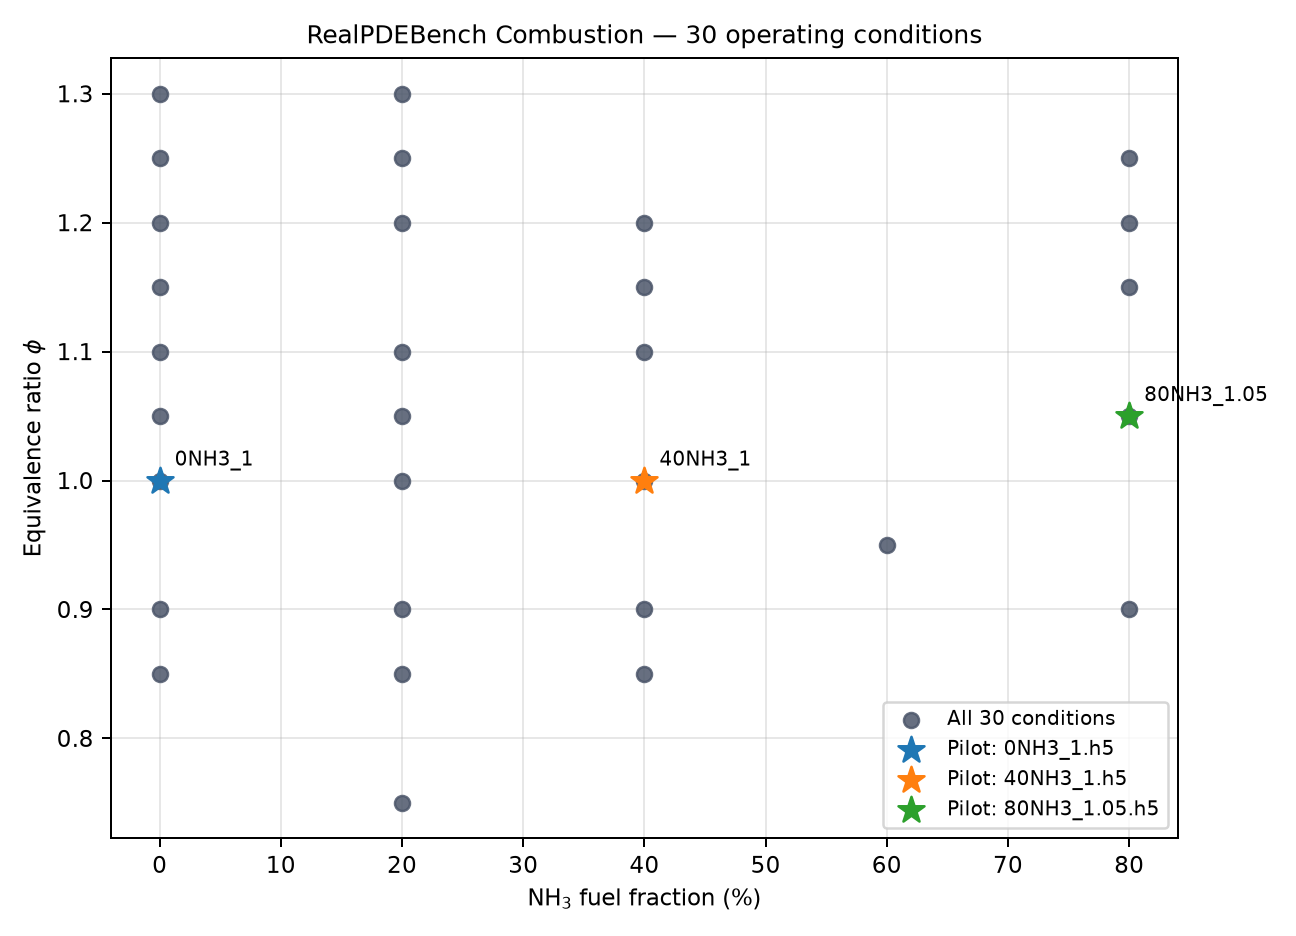
\includegraphics[width=0.74\textwidth]{fig01_parameter_space_30_conditions.png}
    \caption[Operating parameter space of the 30 LES conditions]{Distribution of all 30 numerical LES operating conditions across ammonia fuel fraction ($\text{NH}_3\%$) and equivalence ratio ($\phi$). Highlighted markers indicate the three representative trajectories initially audited in the pilot inspection (\texttt{0NH3\_1.h5}, \texttt{40NH3\_1.h5}, and \texttt{80NH3\_1.05.h5}).}
    \label{fig:data_param_space}
\end{figure}

\subsection{Why Official RealPDEBench Splits Cannot Be Reused Directly}
\label{subsec:data_official_splits}

Inspecting the official index metadata released with \textit{RealPDEBench} (\texttt{train\_\allowbreak{}index\_\allowbreak{}numerical.json}, \texttt{val\_\allowbreak{}index\_\allowbreak{}numerical.json}, and \texttt{test\_\allowbreak{}index\_\allowbreak{}numerical.json}) revealed a structural mismatch with our diagnostic task. In the official benchmark release:
\begin{itemize}
    \item All $30$ numerical conditions ($58{,}860$ temporal windows) are pooled into \texttt{train\_\allowbreak{}index\_\allowbreak{}numerical.json} (\texttt{remain\_\allowbreak{}params\_\allowbreak{}numerical.json} contains 30/30 trajectories), while \texttt{val\_\allowbreak{}index\_\allowbreak{}numerical.json}, \texttt{test\_\allowbreak{}index\_\allowbreak{}numerical.json}, \texttt{in\_\allowbreak{}dist\_\allowbreak{}test\_\allowbreak{}params}, and \texttt{out\_\allowbreak{}dist\_\allowbreak{}test\_\allowbreak{}params} are empty (\texttt{[]} or \texttt{\{\}}). This design reflects \textit{RealPDEBench}'s primary goal: pretraining autoregressive temporal forecasting models ($20 \rightarrow 20$ frames) on half-resolution numerical fields (\texttt{sub\_s = 2}, $64 \times 64$) prior to fine-tuning on experimental line-of-sight $\text{OH}^*$ chemiluminescence sequences ($\sim 3.67\text{ GB}$).
    \item Consequently, reusing the official benchmark indices would test neither cross-variable spatial reconstruction at full $128 \times 128$ resolution (\texttt{sub\_s = 1}) nor generalization to unseen fuel blends and equivalence ratios. This thesis therefore defines its own leakage-free operating-condition split (Section~\ref{sec:data_protocol}).
\end{itemize}

% ==============================================================================
\section{Geometric Orientation, Physical Channels, and Data Quality Audit}
\label{sec:data_geometry}
% ==============================================================================

\subsection{2D Diametral Slice Geometry and Channel Mapping}
\label{subsec:data_geom_channels}

Each Arrow shard stores one complete trajectory at full planar resolution $128 \times 128$ over $2001$ exported snapshots with uniform nominal sampling interval $\Delta t = 2.5 \times 10^{-4}\text{ s}$ ($4000\text{ Hz}$, covering $0.5\text{ s}$ physical duration per trajectory, within absolute simulation windows $t \in [1.5, 2.0]\text{ s}$, $[1.7, 2.2]\text{ s}$, $[3.5, 4.0]\text{ s}$, or $[3.8, 4.3]\text{ s}$). The spatial coordinates are stored as one-dimensional \texttt{float64} arrays of length $128$:
\begin{align}
    x &\in [-0.03691,\; +0.03689]\text{ m} \quad (\text{array axis 1 / columns},\; \Delta x \approx 5.81 \times 10^{-4}\text{ m}), \\
    y &\in [0.06285,\; 0.15913]\text{ m} \quad (\text{array axis 0 / rows},\; \Delta y \approx 7.58 \times 10^{-4}\text{ m}),
\end{align}
spanning a physical observation window of approximately $73.8\text{ mm} \times 96.3\text{ mm}$ located downstream of the burner injector nozzle.

\begin{figure}[H]
    \centering
    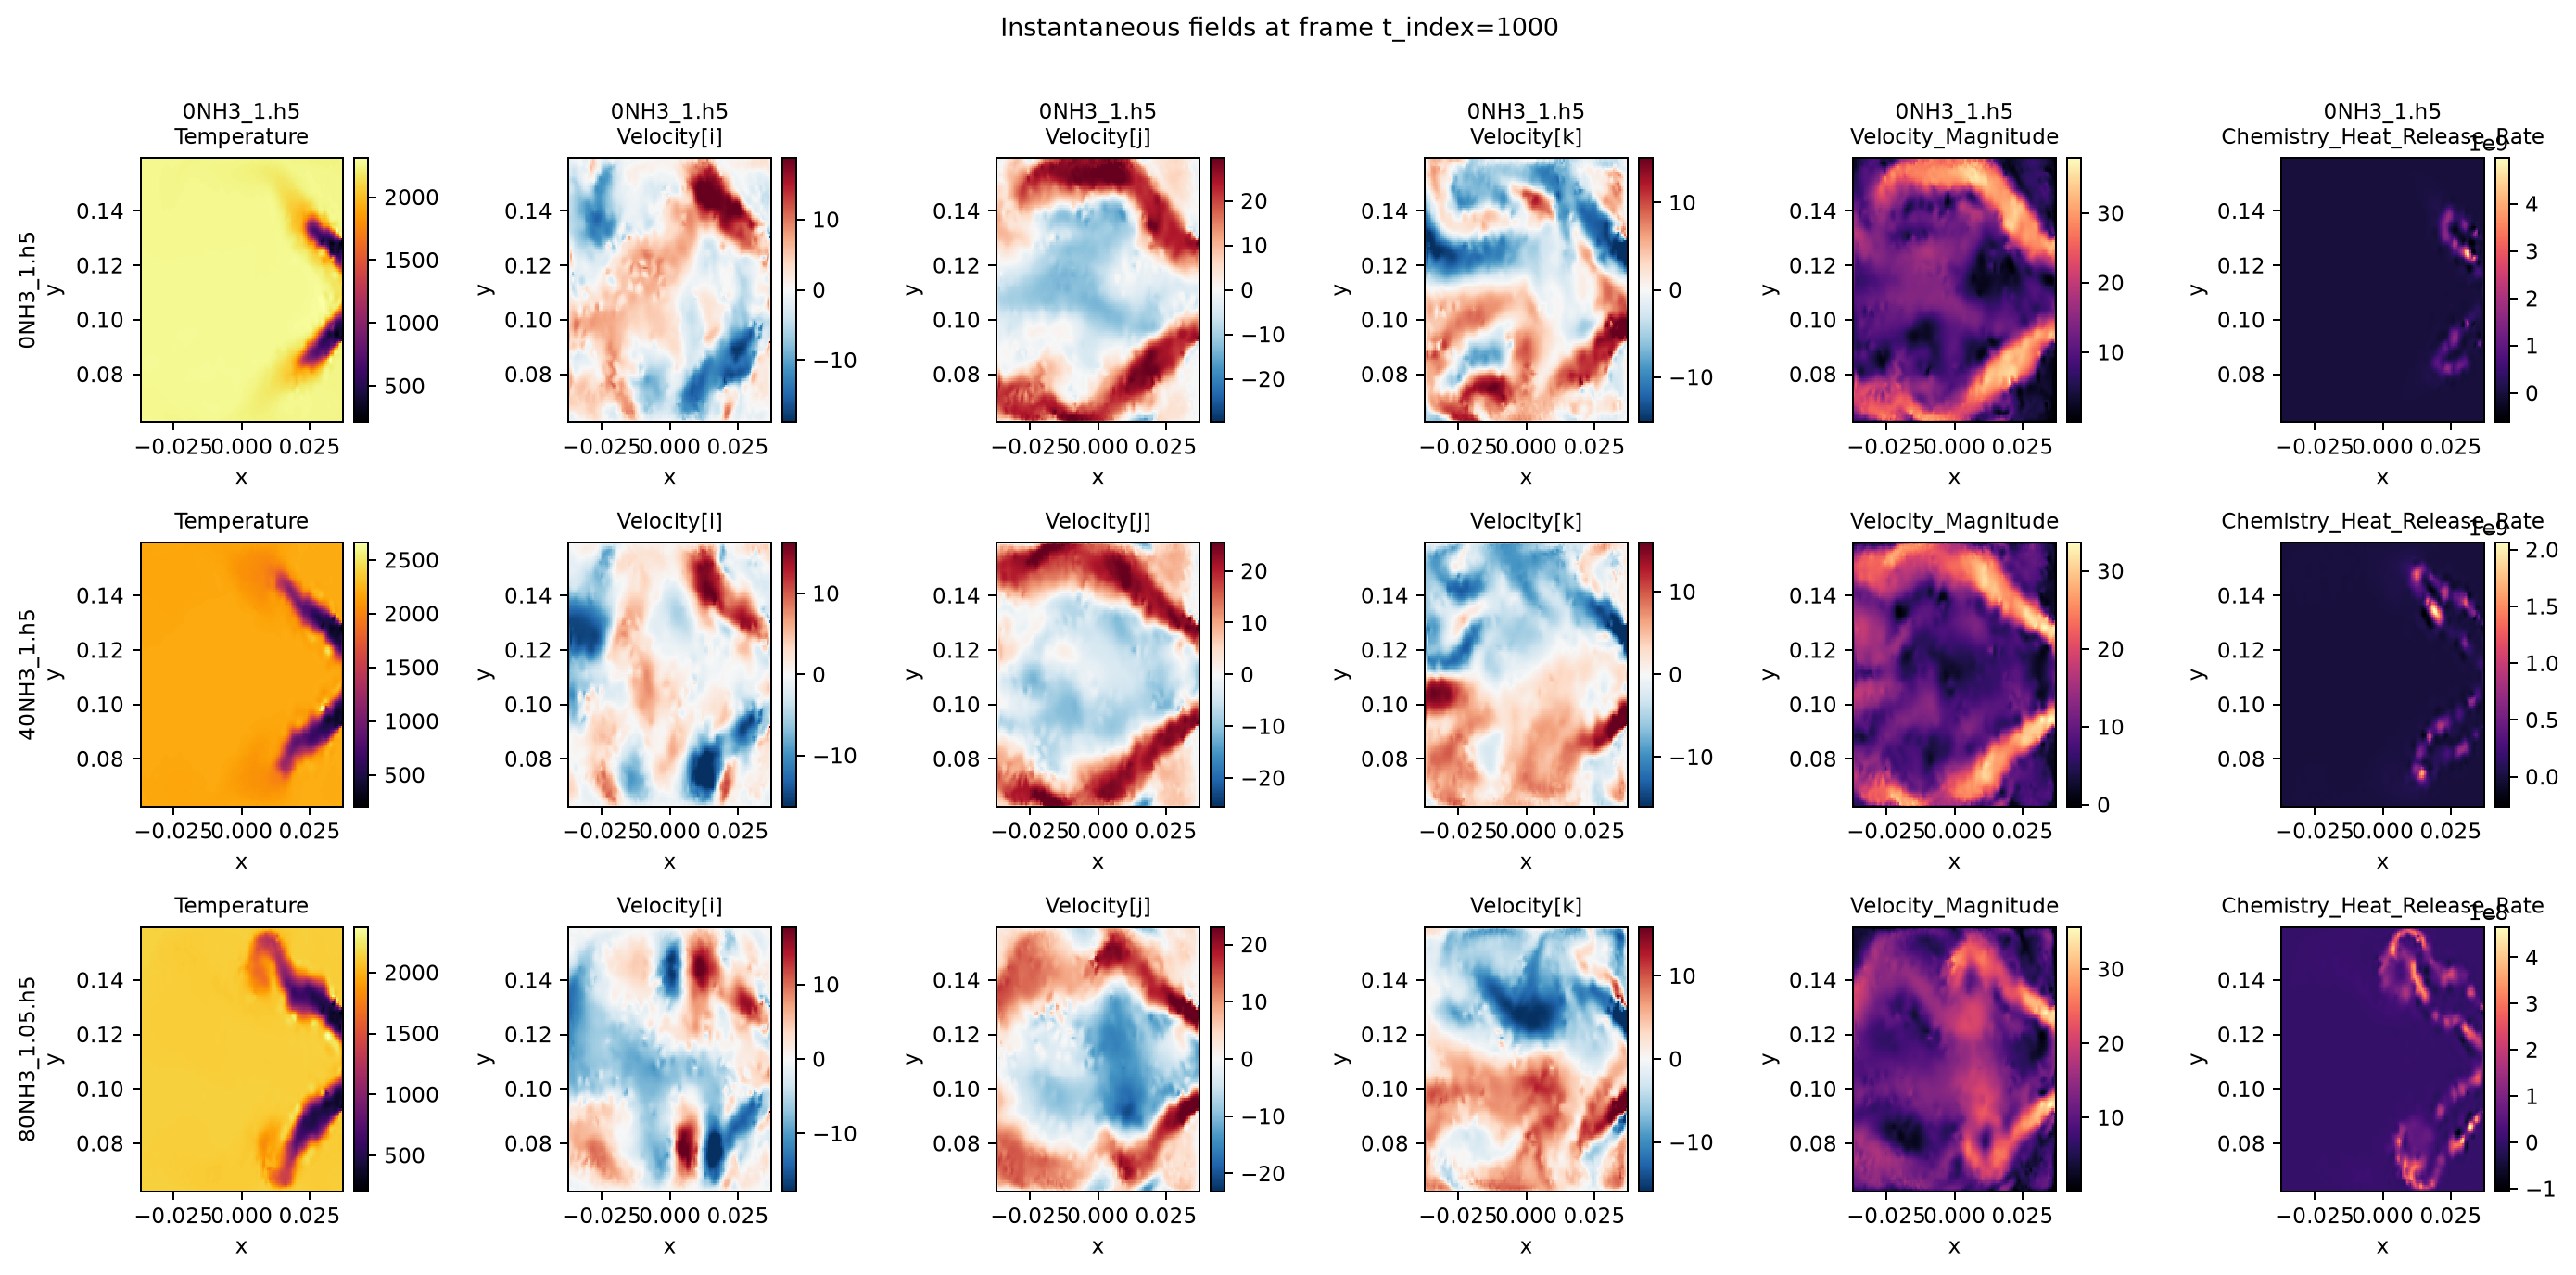
\includegraphics[width=\textwidth]{fig02_pilot_instantaneous_fields.png}
    \caption[Instantaneous physical fields across three representative fuel blends]{Instantaneous LES fields ($T$, $v_i$, $v_j$, $v_k$, exported $|\mathbf{U}|$, and chemical heat release rate) across three pilot operating conditions ($0\%$, $40\%$, and $80\%\text{ NH}_3$ near stoichiometry). Cold reactant jets enter from the right boundary ($x_{\max} \approx +36.9\text{ mm}$) and diverge in a V-shape toward the left, framing the central Inner Recirculation Zone.}
    \label{fig:data_instantaneous}
\end{figure}

\begin{figure}[H]
    \centering
    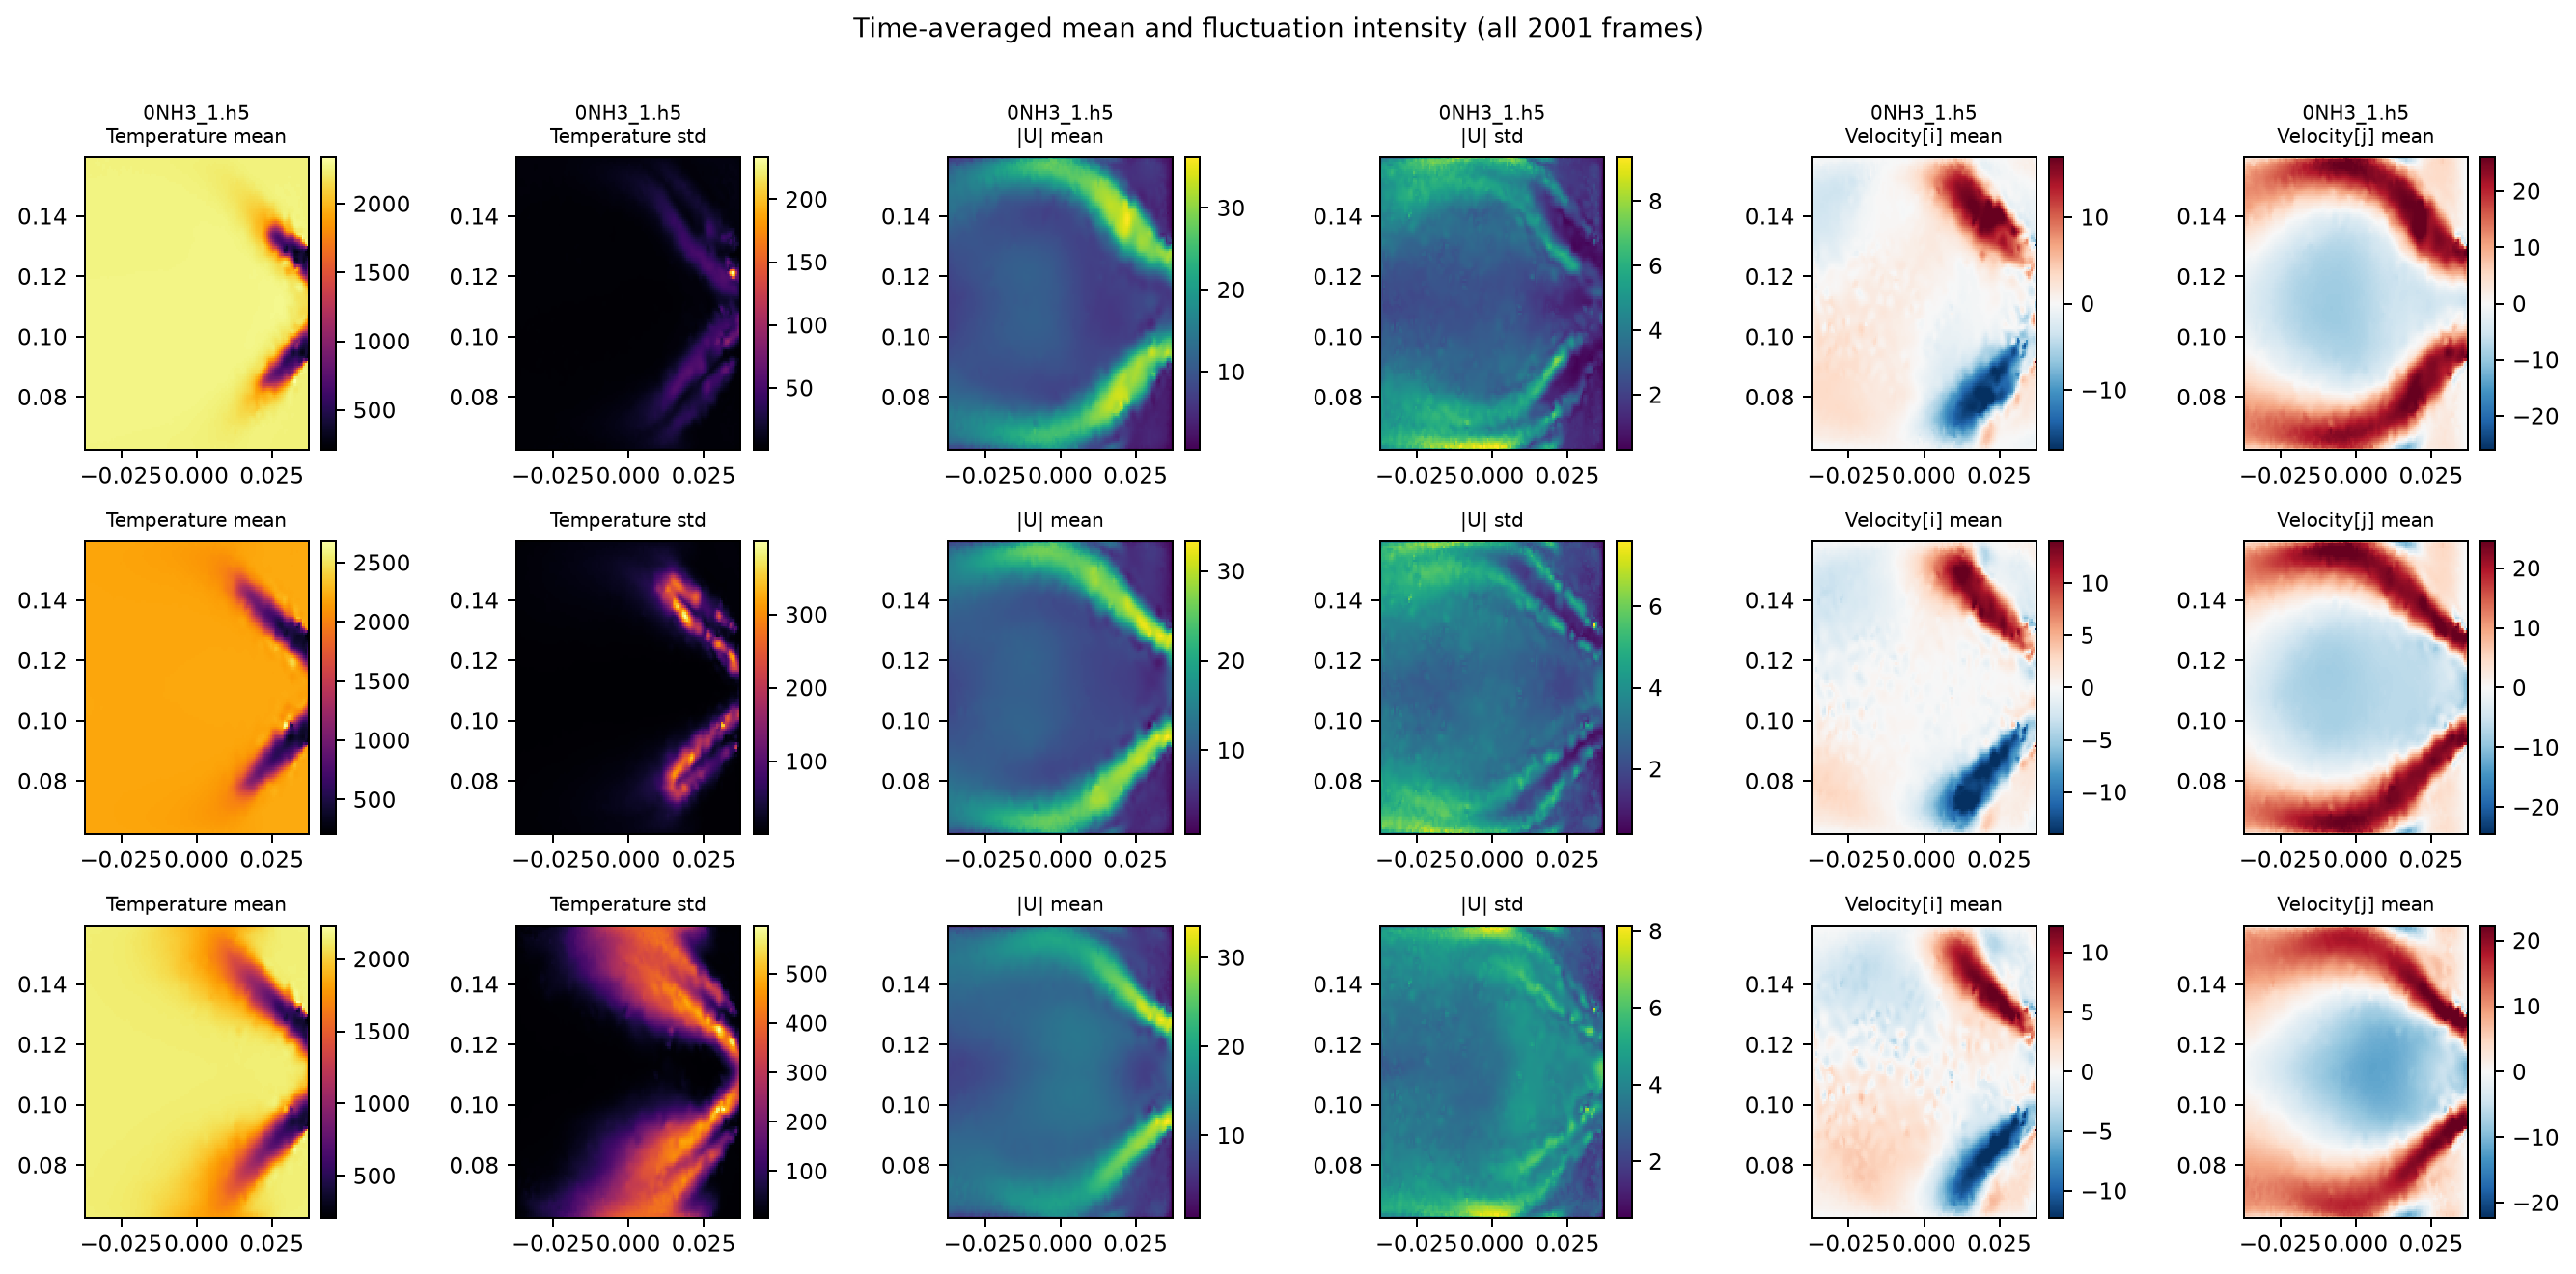
\includegraphics[width=\textwidth]{fig03_pilot_mean_and_std_fields.png}
    \caption[Time-averaged mean and standard deviation of temperature across pilot blends]{Time-averaged mean temperature $\bar{T}$ and temporal standard deviation $\sigma_T$ across the three pilot blends. Peak temperature fluctuations ($\sigma_T \approx 300\text{--}500\text{ K}$) concentrate sharply along the V-shaped shear layers bordering the cold jets, while the interior burnt core remains comparatively uniform.}
    \label{fig:data_mean_std}
\end{figure}

Visual and kinematic inspection of Figures~\ref{fig:data_instantaneous} and~\ref{fig:data_mean_std} establishes the exact physical orientation and channel conventions used throughout this thesis (matching \texttt{channels.json}):
\begin{itemize}
    \item \textbf{Burner symmetry axis and inlet orientation:} The planar field is symmetric about the horizontal centerline near \textbf{row 64} ($y \approx 0.111\text{ m}$). Two cold unburnt reactant branches ($T \approx 300\text{--}400\text{ K}$) enter from the \textbf{right boundary} (\texttt{col = 127}, $x \approx +36.9\text{ mm}$) and diverge radially in a V-shape toward the left (\texttt{col = 0}, $x \approx -36.9\text{ mm}$), enclosing the hot central Inner Recirculation Zone (IRZ). The burner nozzle exit lies immediately outside the cropped field to the right ($x > x_{\max}$).
    \item \textbf{Temperature (Ch~10, target $T$):} Planar LES gas temperature in Kelvin, typically $T \approx 1900\text{--}2280\text{ K}$ inside the burnt recirculation core and $250\text{--}400\text{ K}$ in the incoming reactant cores.
    \item \textbf{Velocity components (Ch~11--13) and directional sign convention:}
    \begin{enumerate}
        \item \texttt{Ch 11 (Velocity[i])}: \textbf{In-plane radial/transverse velocity} $v_i$ [m/s], positive ($+$) in the upper V-branch ($\text{row} > 64$, moving toward $+y$) and negative ($-$) in the lower V-branch ($\text{row} < 64$, moving toward $-y$) as the annular swirling jet expands radially outward.
        \item \texttt{Ch 12 (Velocity[j])}: \textbf{Axial velocity} $v_j$ [m/s], strongly positive ($\sim +20\text{--}30\text{ m/s}$) along the two V-jet branches and negative ($\sim -7\text{ to }-15\text{ m/s}$) inside the central IRZ reverse flow. Crucially, relative to the exported Cartesian grid coordinate $x$, positive $v_j$ points \emph{downstream} toward $-x$ (from right to left); accordingly, physical in-plane streamlines in $(x, y)$ coordinates follow $(-v_j, +v_i)$, and spatial derivatives in $(x, y)$ must respect this sign convention.
        \item \texttt{Ch 13 (Velocity[k])}: \textbf{Out-of-plane azimuthal swirl velocity} $v_k$ [m/s] ($\sim \pm 15\text{ m/s}$), exhibiting antisymmetric signs above and below the symmetry axis (\texttt{row 64}).
    \end{enumerate}
\end{itemize}

\subsection{Data Quality, Physical Guardrails, and Timestamp Anomaly Audit}
\label{subsec:data_quality}

Systematic validation across all $30$ shards ($\sim 9.83 \times 10^8$ space--time grid points) verified zero \texttt{NaN} or \texttt{Inf} entries in any tensor, while uncovering four dataset anomalies that govern how the preprocessing pipeline handles the raw arrays:
\begin{enumerate}
    \item \textbf{Artifacts in exported \texttt{Velocity\_Magnitude} (Ch~14):} Comparison between the exported Ch~14 array and the exact Euclidean norm $|\mathbf{u}| = \sqrt{v_i^2 + v_j^2 + v_k^2}$ computed from Ch~11--13 reveals small numerical interpolation artifacts in Ch~14, including unphysical negative magnitudes down to $-8\text{ m/s}$. Our pipeline therefore discards Ch~14 and always recomputes velocity magnitude directly from the orthogonal velocity components.
    \item \textbf{Rare temperature interpolation outliers (Ch~10):} While the bulk temperature field lies strictly within physical combustion bounds ($[250, 2350]\text{ K}$), grid resampling from the unstructured 3D LES mesh onto the $128 \times 128$ Cartesian slice introduces rare isolated undershoots ($T < 0\text{ K}$ in $15/30$ conditions, typically $10\text{--}600$ voxels out of $3.28 \times 10^7$ per condition, i.e., $\ll 0.01\%$, worst $-375\text{ K}$) and overshoots ($T > 2600\text{ K}$ in $24/30$ conditions, $< 0.03\%$ of voxels, up to $3002\text{ K}$). To maintain transparent target continuity, raw Ch~10 temperatures are preserved without silent clipping during baseline benchmarking, while sensitivity to physical clipping is flagged as a protocol check.
    \item \textbf{Separation of planar $\text{OH}$ (Ch~8) and experimental $\text{OH}^*$ (\texttt{observed}):} In \textit{RealPDEBench}, the \texttt{observed} array represents line-of-sight integrated $\text{OH}^*$ chemiluminescence intensity (mapped from numerical fields by the benchmark's surrogate network), whereas Ch~8 (\texttt{Mole\_Fraction\_of\_OH}) is the 2D planar LES species concentration. Neither channel is ever conflated with the other or passed into velocity-to-temperature inputs.
    \item \textbf{Interior timestamp gap and duplicate frame in \texttt{40NH3\_1.2.h5} (shard \texttt{data-00022-of-00030.arrow}):} A fine-grained timeline audit conducted during pipeline hardening established that while the numerical tensor of \texttt{40NH3\_1.2.h5} has shape $(2001, 128, 128, 15)$, its exported time coordinate array \texttt{t} contains only $2000$ entries spanning $[1.5, 2.0]\text{ s}$ with a single interior step doubling ($\Delta t_{1098} \approx 5.0 \times 10^{-4}\text{ s}$ corresponding to deletion of uniform index $1099$) and bitwise-identical field snapshots at indices $1999$ and $2000$. Consequently, single-frame instantaneous reconstruction indexed by snapshot ID remains valid, whereas unverified multi-frame or temporal forecasting evaluation on this shard is explicitly blocked by dataset metadata flags (\texttt{field\_time\_association\_verified = False}).
\end{enumerate}

% ==============================================================================
\section{Thermodynamic Trends, Temporal Autocorrelation, and Kinematic Coupling}
\label{sec:data_coupling}
% ==============================================================================

\subsection{Parametric Trends Across the 30 Operating Conditions}
\label{subsec:data_trends}

Figure~\ref{fig:data_trends} summarizes how key thermal and kinematic quantities vary across the 30 conditions as functions of $\text{NH}_3\%$ and $\phi$:
\begin{itemize}
    \item \textbf{Systematic cooling and deeper cold-jet penetration with ammonia blending:} At matched equivalence ratio $\phi$, domain-mean temperature drops by $185\text{--}225\text{ K}$ from $0\%\text{ NH}_3$ ($\bar{T} = 2000.4\text{--}2186.5\text{ K}$) to $80\%\text{ NH}_3$ ($\bar{T} = 1864.5\text{--}1957.2\text{ K}$), while the mean volume fraction of cold unburnt pockets ($T < 1200\text{ K}$) more than doubles from $3.5\%$ to $8.5\%$. Within each fixed $\text{NH}_3$ band, $\bar{T}$ peaks near $\phi \approx 1.0\text{--}1.05$ and decreases sharply toward both lean ($\phi = 0.75$) and rich ($\phi = 1.25\text{--}1.30$) limits, reflecting lower heat release and chemical dilution. Meanwhile, fully burnt gases ($T > 1800\text{ K}$) occupy $81\%\text{--}96\%$ of the observation window across all 30 conditions.
    \item \textbf{Bulk velocity trends:} Across $28$ of the $30$ conditions, recomputed mean flow speed $\overline{|\mathbf{u}|}$ remains tightly clustered between $10.0$ and $14.9\text{ m/s}$, generally decreasing with increasing $\phi$ within each fuel blend ($r \in [-0.76, -0.99]$, with a slight upward inflection at $\phi = 1.2$ in $20\%\text{ NH}_3$). Two lean pure-methane trajectories (\texttt{0NH3\_0.85} and \texttt{0NH3\_0.90}) exhibit noticeably higher bulk flow speeds ($23.77$ and $17.3\text{ m/s}$, respectively), consistent with inflow mass-flow adjustments used to vary $\phi$ in those operating points.
\end{itemize}

\begin{figure}[H]
    \centering
    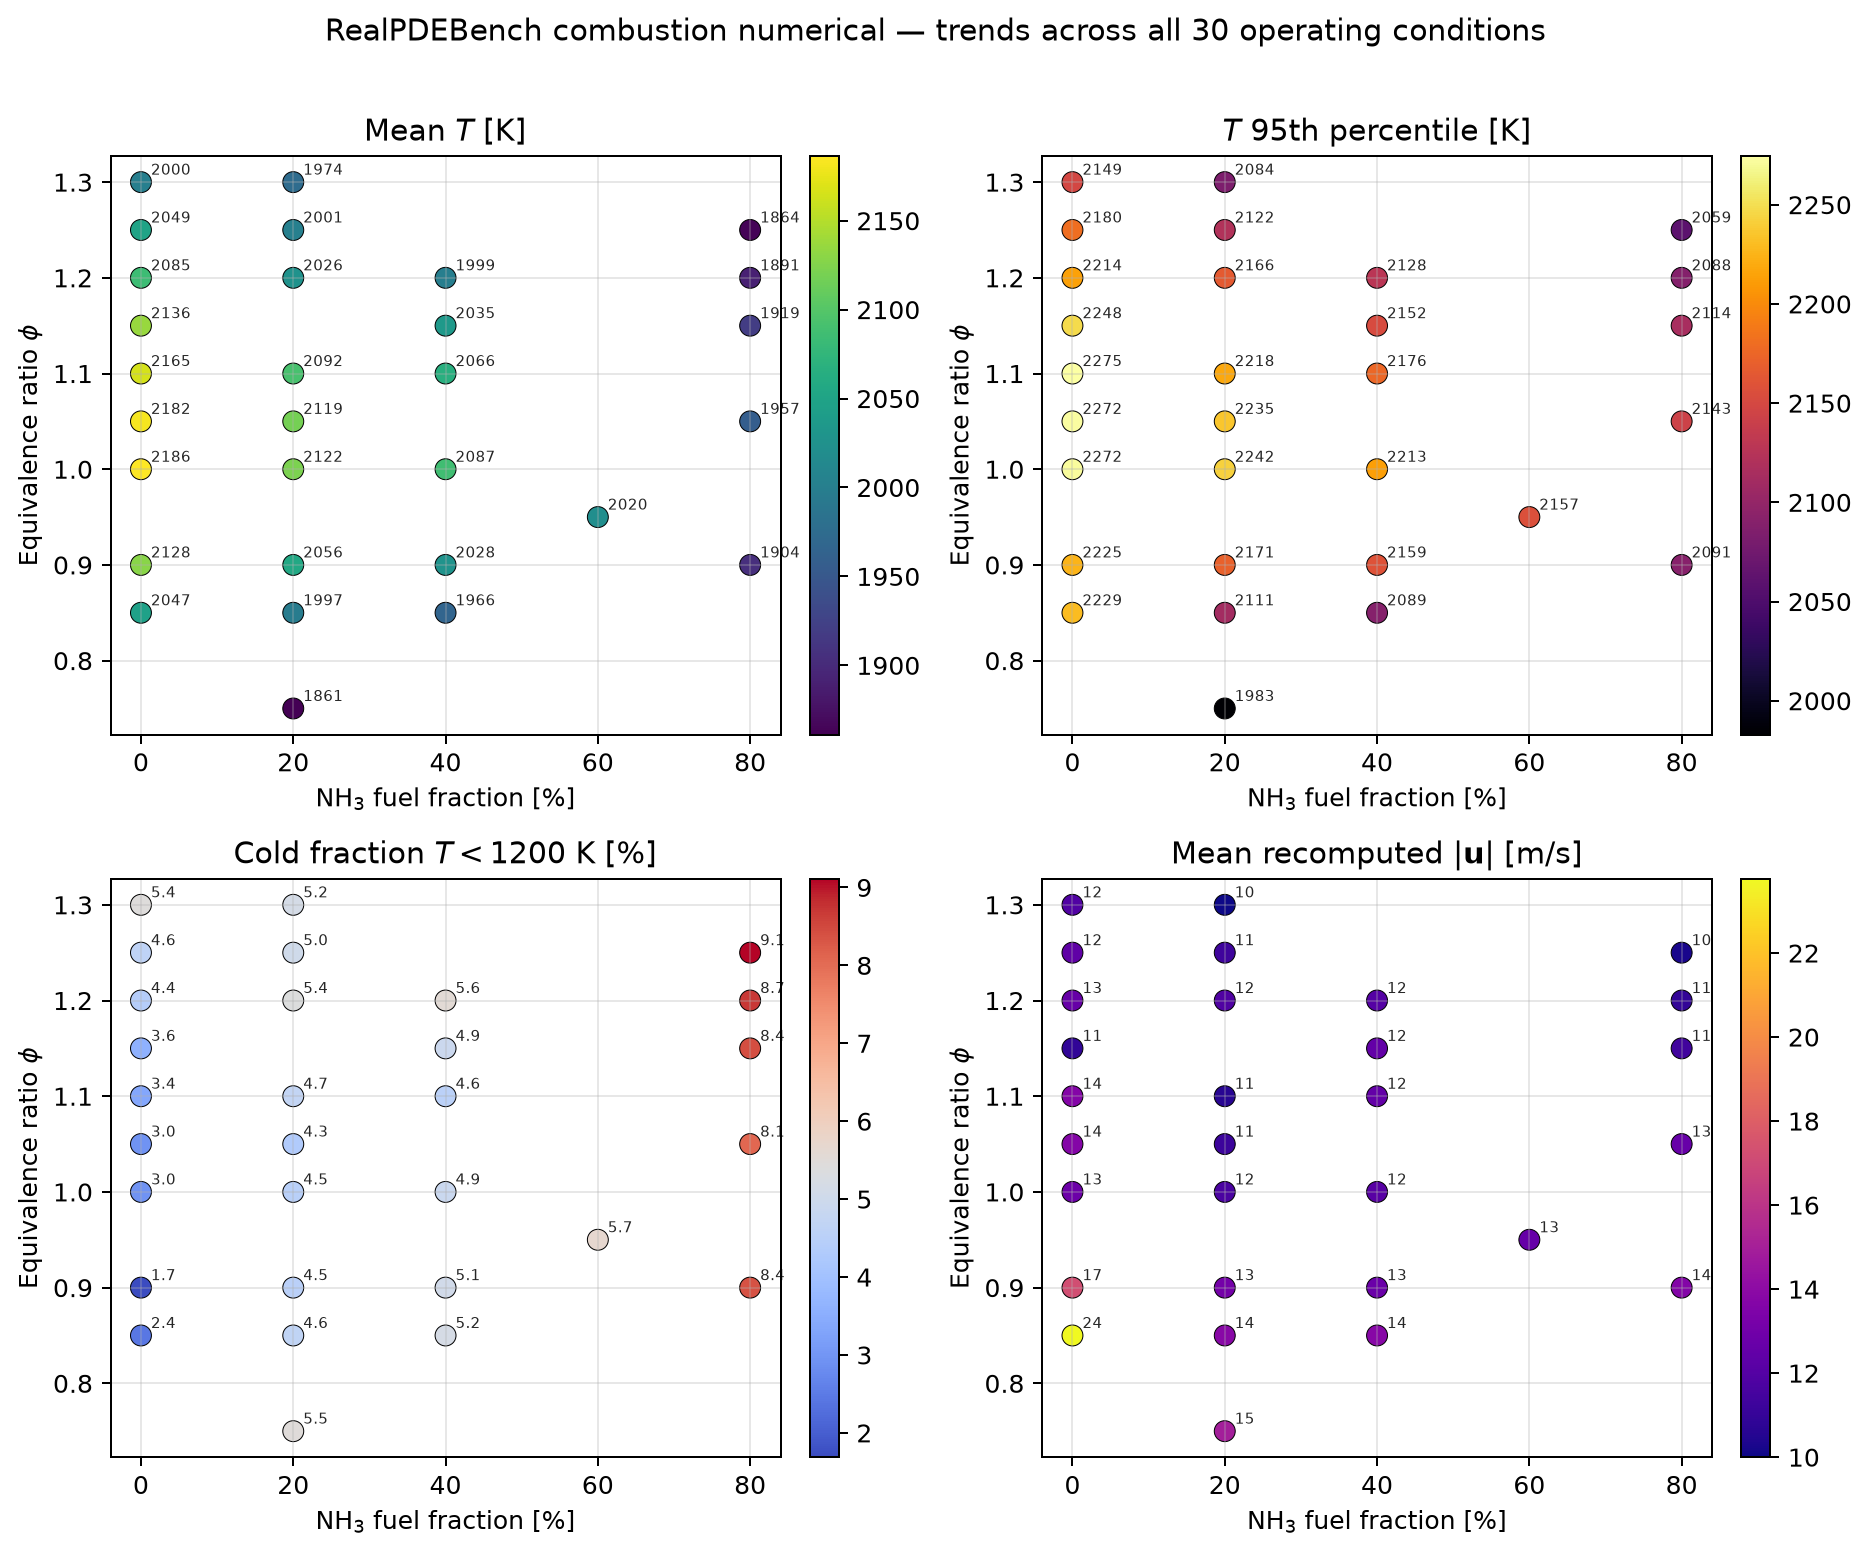
\includegraphics[width=0.96\textwidth]{fig05_all30_temperature_velocity_trends.png}
    \caption[Thermodynamic and kinematic trends across all 30 LES operating conditions]{Trends across all 30 LES operating conditions vs.\ equivalence ratio $\phi$, grouped by $\text{NH}_3\%$ fraction: domain-mean temperature $\bar{T}$, 95th-percentile temperature $T_{p95}$, cold reactant fraction ($T < 1200\text{ K}$), and recomputed mean velocity magnitude $\overline{|\mathbf{u}|}$.}
    \label{fig:data_trends}
\end{figure}

\subsection{Temperature Histograms and Flame-Brush Temporal Autocorrelation}
\label{subsec:data_autocorr}

Figure~\ref{fig:data_hist_autocorr} examines the marginal temperature distributions and temporal decorrelation timescales on the three pilot trajectories. Across all blends, the temperature histogram is strongly bimodal and burnt-dominated: a sharp peak centered around $2050\text{--}2250\text{ K}$ accounts for roughly $90\%$ of space--time voxels, accompanied by a long low-temperature shoulder ($300\text{--}1800\text{ K}$) corresponding to the cold annular jets and reaction mixing layer whose weight expands systematically with $\text{NH}_3\%$. Along the transverse midline cut (Figure~\ref{fig:data_hist_autocorr}, panel a2), the radial temperature profile shows two symmetric cold dips near rows $\sim 40$ and $\sim 88$ corresponding to the upper and lower branches of the annular jet.

\begin{figure}[H]
    \centering
    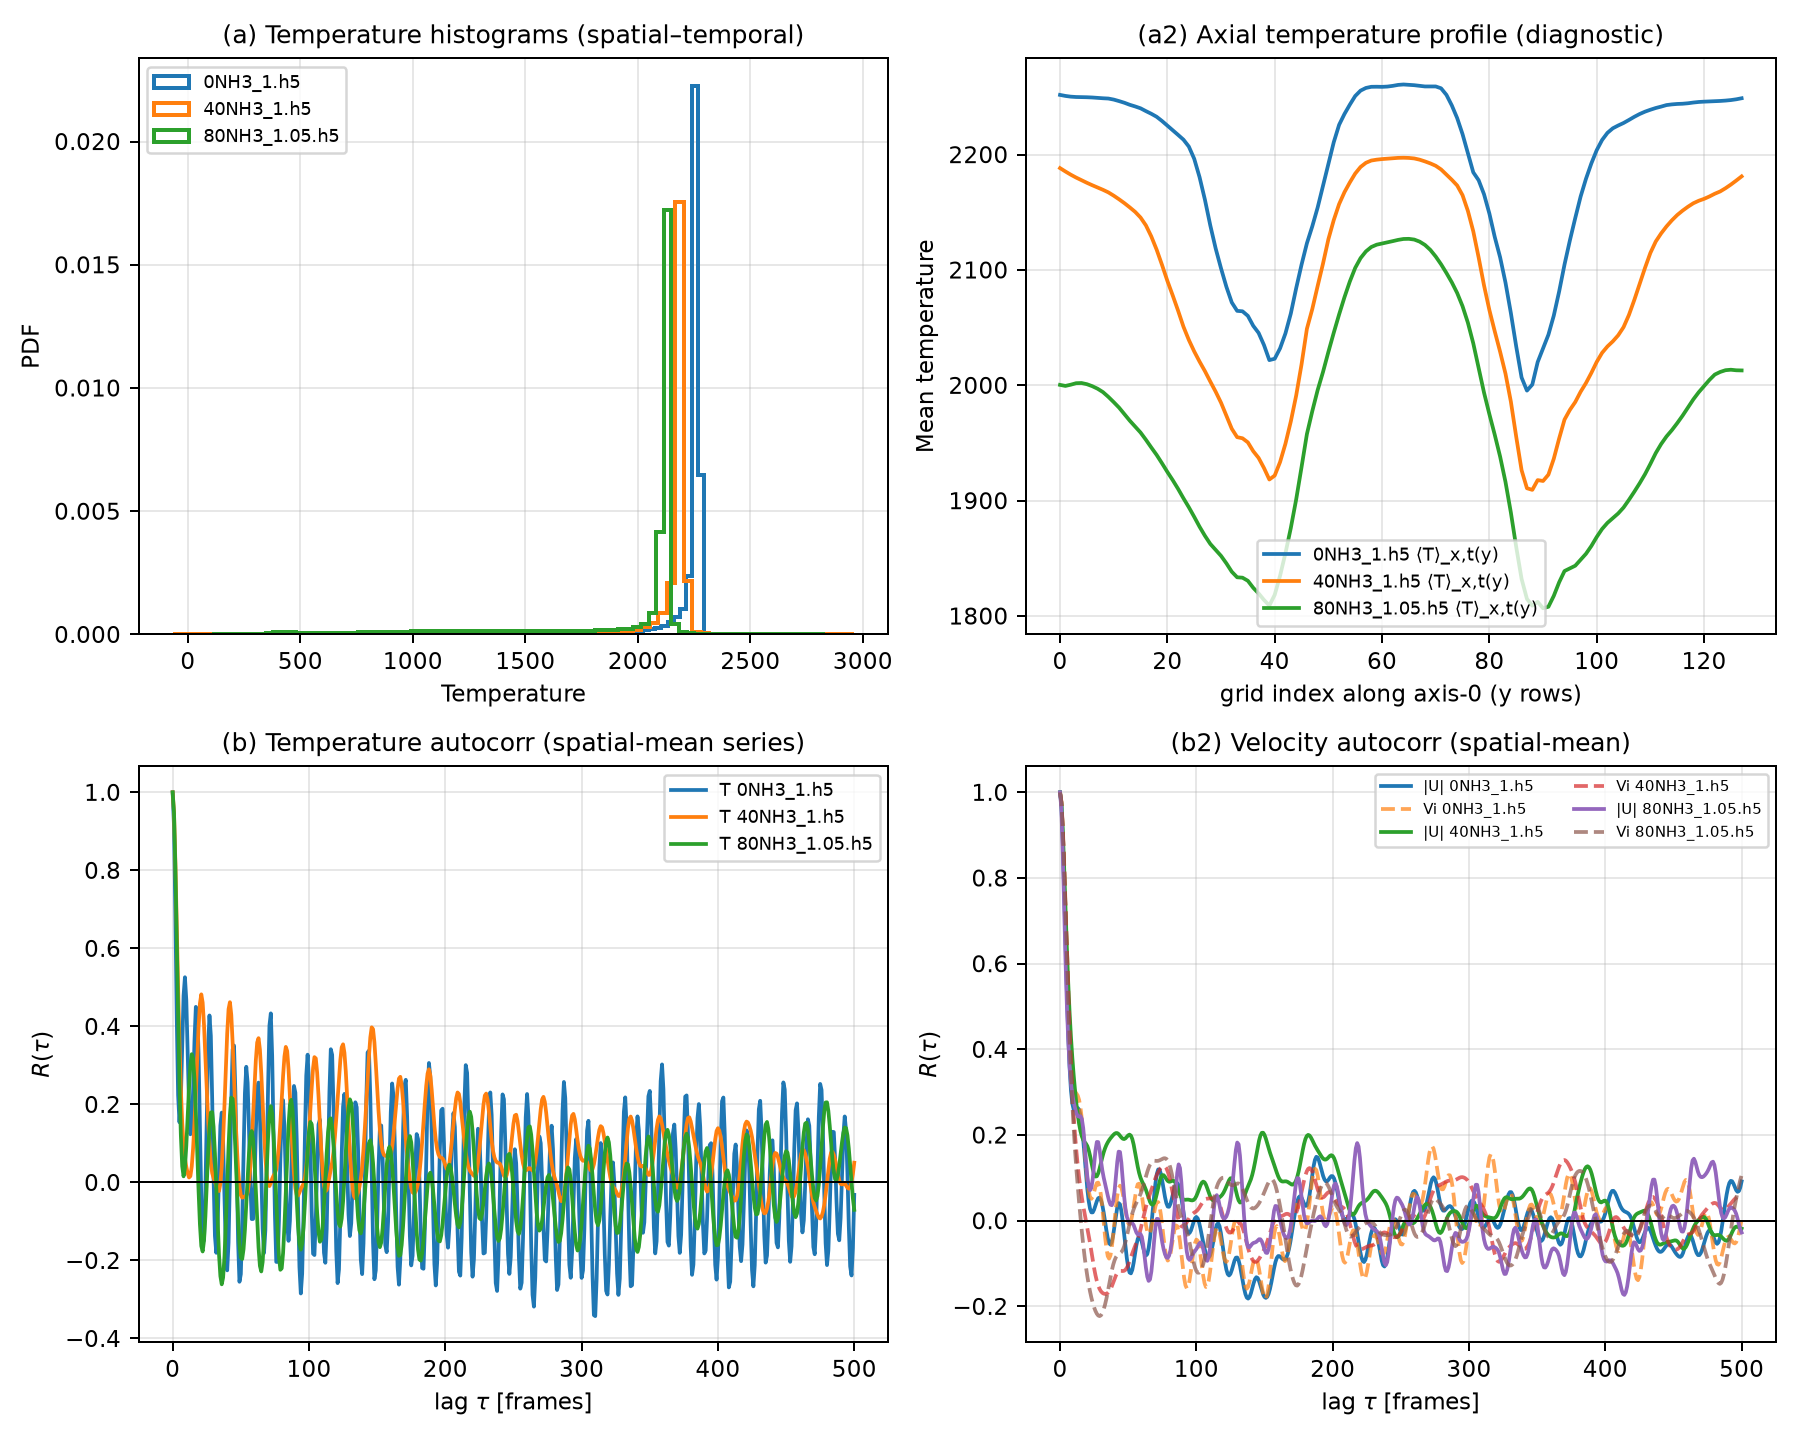
\includegraphics[width=\textwidth]{fig04_temperature_histograms_and_autocorr.png}
    \caption[Temperature distributions and temporal autocorrelation timescales]{(a1--a2)~Temperature distributions and mean radial profiles across rows ($y$) showing symmetric cold jet dips near rows $40$ and $88$. (b1--b2)~Temporal autocorrelation functions $R(\Delta t)$ of domain-mean temperature versus high-variance flame-brush points: local flame-front fluctuations remain correlated over $50\text{--}100+$ frames ($\tau_c \approx 14\text{ ms}$).}
    \label{fig:data_hist_autocorr}
\end{figure}

Crucially, panel~(b) of Figure~\ref{fig:data_hist_autocorr} reveals a two-scale temporal decorrelation structure. While the domain-averaged temperature decays over $O(10\text{--}20)$ frames ($\sim 2.5\text{--}5\text{ ms}$), individual spatial locations inside the high-variance flame brush retain significant temporal correlation across \textbf{$50\text{--}100+$ consecutive frames} ($\tau_c \approx 14\text{ ms}$ at $4000\text{ Hz}$). Splitting frames randomly within a single trajectory would therefore place nearly identical flame snapshots in both training and test sets, inflating apparent generalization through temporal memorization.

\subsection{Kinematic--Thermal Coupling and Cross-Condition Ambiguity}
\label{subsec:data_kinematic_check}

Before fitting any reconstruction model, we quantified the physical coupling between velocity features (and spatial velocity derivatives) and temperature across the 20 training trajectories (\texttt{Check 1}, Table~\ref{tab:data_check1} and Figure~\ref{fig:data_check1}):

\begin{table}[H]
\centering
\caption[Pointwise kinematic--thermal correlations with temperature]{Pointwise correlations between velocity / kinematic gradient features and temperature $T$ across the 20 training conditions (\texttt{Check 1}), comparing pooled multi-condition statistics (Pearson $r$, Spearman $\rho$, and mutual information MI) against within-condition Pearson $r$ (mean $\pm$ std across the 20 trajectories).}
\label{tab:data_check1}
\small
\resizebox{\textwidth}{!}{%
\begin{tabular}{lrrrr}
\toprule
\textbf{Feature} & \textbf{Pooled Pearson $r$} & \textbf{Pooled Spearman $\rho$} & \textbf{Pooled MI} & \textbf{Within-Cond. Pearson $r$} \\
\midrule
Velocity magnitude $|\mathbf{u}|$ & $-0.3788$ & $-0.2798$ & $0.1169$ & $-0.474 \pm 0.114$ \\
Axial velocity $v_j$ & $-0.3196$ & $-0.2057$ & $0.1282$ & $-0.384 \pm 0.120$ \\
Strain-rate magnitude $\|S_{\text{2D}}\|$ & $-0.1231$ & $-0.1302$ & $0.0224$ & $-0.250 \pm 0.091$ \\
Out-of-plane vorticity $|\omega_z|$ & $-0.0643$ & $-0.0639$ & $0.0175$ & $-0.198 \pm 0.058$ \\
Planar dilatation $\nabla_{\text{2D}}\cdot\mathbf{u}$ & $-0.0204$ & $+0.0092$ & $0.0125$ & $-0.025 \pm 0.060$ \\
Azimuthal swirl $v_k$ & $+0.0103$ & $+0.0173$ & $0.0778$ & $+0.004 \pm 0.014$ \\
Radial velocity $v_i$ & $+0.0065$ & $+0.0141$ & $0.0706$ & $+0.003 \pm 0.024$ \\
\bottomrule
\end{tabular}%
}
\end{table}

\begin{figure}[H]
    \centering
    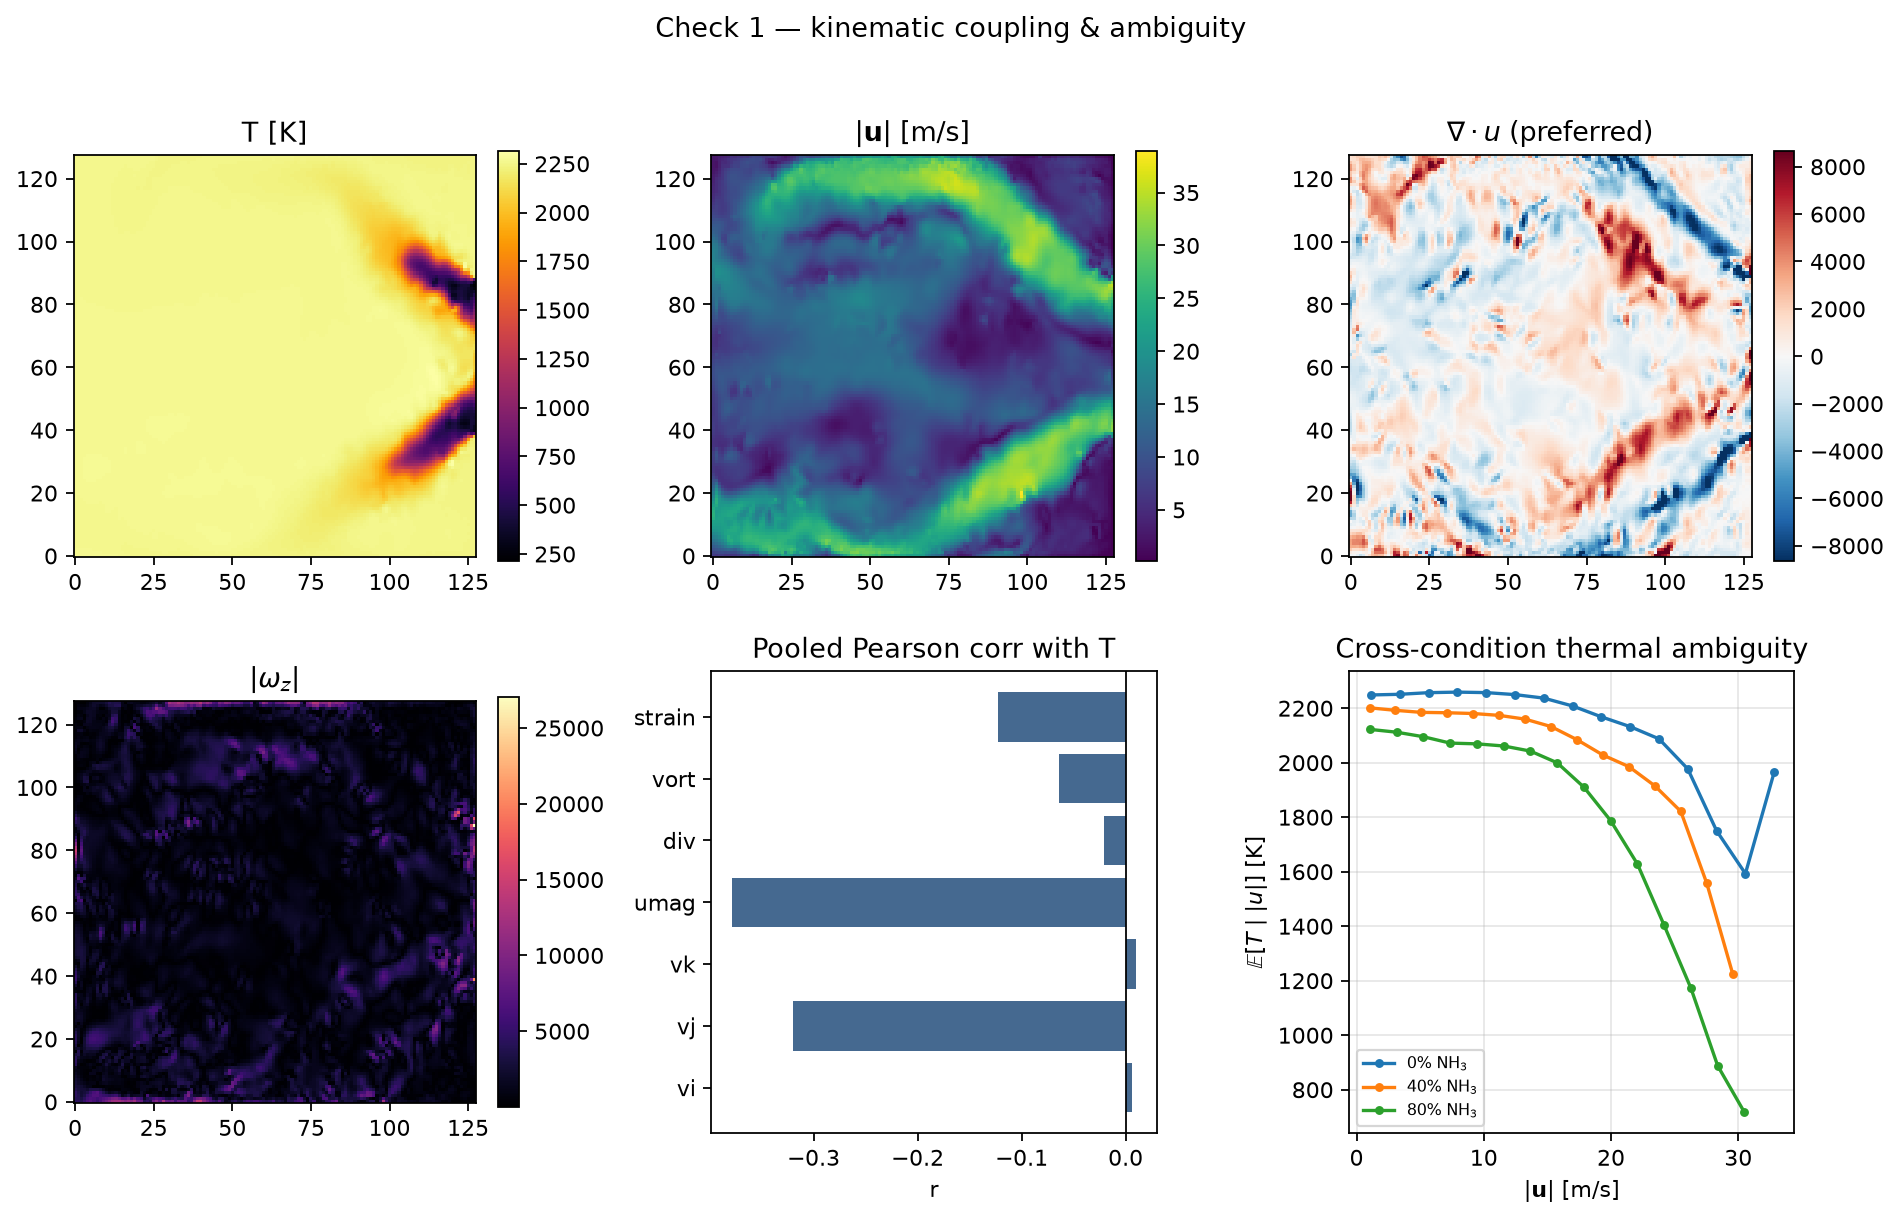
\includegraphics[width=\textwidth]{fig07_kinematic_coupling_and_ambiguity.png}
    \caption[Kinematic--thermal coupling and cross-condition thermal ambiguity]{Physical feasibility analysis (\texttt{Check 1}): instantaneous $T$, $|\mathbf{u}|$, planar dilatation $\nabla_{\text{2D}}\cdot\mathbf{u}$, and vorticity $|\omega_z|$ on a stoichiometric methane snapshot (\texttt{0NH3\_1.h5}), alongside pooled Pearson correlations with $T$ and conditional expectation curves $\mathbb{E}[T \mid |\mathbf{u}|]$ across $0\%$, $40\%$, and $80\%\text{ NH}_3$ blends.}
    \label{fig:data_check1}
\end{figure}

Table~\ref{tab:data_check1} and Figure~\ref{fig:data_check1} establish three essential physical properties of the inverse problem:
\begin{enumerate}
    \item \textbf{Within-condition spatial localization:} Within any fixed operating condition, velocity magnitude $|\mathbf{u}|$ ($r = -0.474 \pm 0.114$) and axial velocity $v_j$ ($r = -0.384 \pm 0.120$) correlate strongly and negatively with temperature because high-momentum V-jets transport cold reactants whereas low-speed recirculation cores hold hot burnt gas. Notice that $v_i$ and $v_k$ show near-zero linear correlation with $T$ solely because they are antisymmetric about the burner axis (\texttt{row 64}) while $T$ is symmetric---yet they carry significant mutual information ($\text{MI} = 0.071\text{--}0.078$).
    \item \textbf{Cross-condition thermodynamic confounding:} Pooling samples across all 20 conditions weakens the linear correlation ($|\mathbf{u}|$: $-0.474 \rightarrow -0.379$), and the conditional expectation curves $\mathbb{E}[T \mid |\mathbf{u}|]$ (Figure~\ref{fig:data_check1}, bottom right) separate vertically by \textbf{$200\text{--}360\text{ K}$} between $0\%$, $40\%$, and $80\%\text{ NH}_3$ at identical local flow speeds (e.g., $\sim 2150\text{ K}$ vs.\ $\sim 1800\text{ K}$ at $|\mathbf{u}| = 20\text{ m/s}$). Local velocity observations alone are therefore thermodynamically ambiguous without knowledge of $\mathbf{p} = (\text{NH}_3\%, \phi)$ or sparse temperature anchors.
    \item \textbf{Thin-sheet localization of planar dilatation:} Pointwise planar divergence $\nabla_{\text{2D}}\cdot\mathbf{u}$ has near-zero correlation with bulk temperature $T$ ($r = -0.0204$), whereas on the representative \texttt{0NH3\_1.h5} snapshot the magnitude $|\nabla_{\text{2D}}\cdot\mathbf{u}|$ correlates positively with the flame-front temperature gradient $|\nabla T|$ ($r = +0.2368$). Consistent with the low-Mach physics in Section~\ref{sec:bg_pinns}, dilatation is concentrated along the thin reaction sheet (and polluted by unclosed $\partial_z v_k$ out-of-plane swirl divergence) rather than varying proportionally with bulk $T$.
\end{enumerate}

% ==============================================================================
\section{Locked Operating-Condition Splits and Decomposed Evaluation Protocol}
\label{sec:data_protocol}
% ==============================================================================

\subsection{Condition-Level Partition and Temporal Protocol}
\label{subsec:data_splits}

To eliminate trajectory-level leakage across the $50\text{--}100$ frame correlation horizon, all $30$ operating conditions are partitioned strictly at the trajectory level into four disjoint splits (\texttt{configs/splits/splits\_interp\_extrap.yaml}, Figure~\ref{fig:data_splits}):

\begin{table}[H]
\centering
\caption[Locked operating-condition partition across the 30 LES trajectories]{Locked operating-condition split across the 30 LES simulations ($20+3+3+4 = 30$, zero overlap). Within each training condition, fit and seen-evaluation temporal indices are separated by a $120$-frame ($\ge 2\tau_c$) buffer.}
\label{tab:data_splits}
\small
\resizebox{\textwidth}{!}{%
\begin{tabular}{lrp{6.8cm}p{4.3cm}}
\toprule
\textbf{Split} & \textbf{\# Cond.} & \textbf{Assigned Operating Conditions (\texttt{sim\_id})} & \textbf{Scientific Role} \\
\midrule
\texttt{train} & 20 & \texttt{0NH3}: $0.85, 0.90, 1.00, 1.10, 1.15, 1.20, 1.25$; \newline \texttt{20NH3}: $0.85, 0.90, 1.05, 1.20, 1.25$; \newline \texttt{40NH3}: $0.85, 1.00, 1.10, 1.20$; \newline \texttt{80NH3}: $0.90, 1.05, 1.15, 1.20$ & Model fitting (\texttt{train\_fit}: frames $0\text{:}1480\text{:}40$, 38/traj = 760) and seen diagnostics (\texttt{seen\_train\_eval}: frames $1600\text{:}2000\text{:}40$, 11/traj = 220) \\
\midrule
\texttt{val} & 3 & \texttt{0NH3\_1.05}, \texttt{20NH3\_1.10}, \texttt{40NH3\_0.90} & Architecture and hyperparameter selection (frames $0\text{:}2000\text{:}50$, 41/traj = 123) \\
\midrule
\texttt{test\_interp} & 3 & \texttt{20NH3\_1.00}, \texttt{40NH3\_1.15}, \texttt{60NH3\_0.95} & Held-out transfer strictly inside the $(\text{NH}_3\%, \phi)$ training hull (including unseen $60\%\text{ NH}_3$ blend; 41/traj = 123) \\
\midrule
\texttt{test\_extrap} & 4 & \texttt{20NH3\_0.75} (leanest), \texttt{0NH3\_1.30}, \texttt{20NH3\_1.30} (richest), \texttt{80NH3\_1.25} (high-$\text{NH}_3$ rich corner) & Held-out boundary and out-of-range generalization (41/traj = 164) \\
\bottomrule
\end{tabular}%
}
\end{table}

\begin{figure}[H]
    \centering
    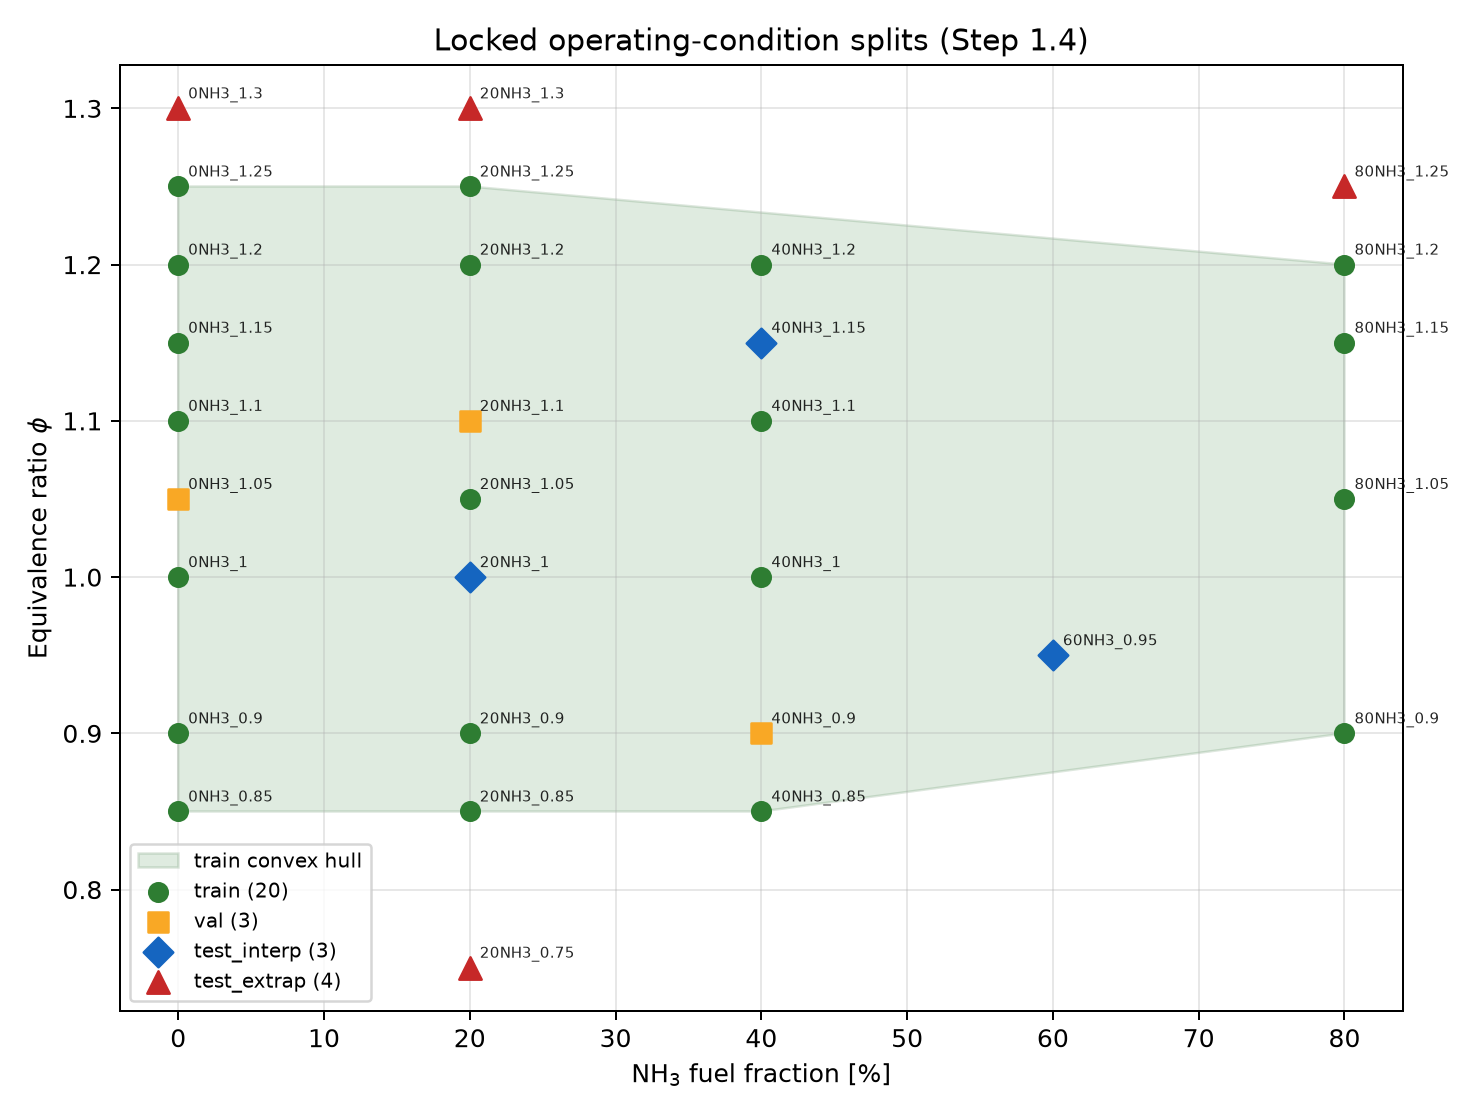
\includegraphics[width=0.66\textwidth]{fig06_locked_operating_condition_splits.png}
    \caption[Locked operating-condition splits across the parameter space]{Locked partition of the 30 operating conditions into \texttt{train} (20), \texttt{val} (3), \texttt{test\_interp} (3), and \texttt{test\_extrap} (4), with the shaded polygon indicating the training convex hull.}
    \label{fig:data_splits}
\end{figure}

As detailed in Table~\ref{tab:data_splits}, all held-out conditions (\texttt{val}, \texttt{test\_interp}, \texttt{test\_extrap}) remain strictly disjoint from training. Inside the 20 training trajectories, models are fit exclusively on the first 75\% of each simulation (\texttt{train\_fit}: frame indices $0\text{--}1480$ strided by $40$, yielding $760$ snapshots), whereas seen-condition diagnostics are evaluated on the final 20\% (\texttt{seen\_train\_eval}: frame indices $1600\text{--}2000$ strided by $40$, yielding $220$ snapshots) after a $120$-frame ($30\text{ ms} \ge 2\tau_c$) separation buffer.

\subsection{Fit-Only Normalization Statistics}
\label{subsec:data_normalization}

All field z-score normalizations ($\tilde{q} = (q - \mu_q) / \sigma_q$) and operating-parameter scalings are computed exclusively on training data without touching \texttt{val} or \texttt{test} trajectories. Table~\ref{tab:data_norm_stats} compares the initial Month-1 training-condition statistics (all $2001$ frames of the $20$ training trajectories) against the tightened Month-2 \texttt{train\_fit}-only statistics restricted strictly to the $760$ fit frames ($0\text{--}1480$): excluding the seen-evaluation block alters $\mu_T$ and $\sigma_T$ by less than $0.3\text{ K}$ ($0.05\%$) while guaranteeing zero temporal leakage into normalization constants.

\begin{table}[H]
\centering
\caption[Training-only normalization statistics]{Training-only normalization statistics (Welford online unclipped mean and standard deviation) across the 20 training conditions, comparing all-frame training statistics (\texttt{train\_\allowbreak{}norm\_\allowbreak{}stats.json}) against the strict \texttt{train\_fit}-only statistics (\texttt{train\_\allowbreak{}norm\_\allowbreak{}stats\_\allowbreak{}month2\_\allowbreak{}fit.json}, 760 snapshots).}
\label{tab:data_norm_stats}
\small
\resizebox{\textwidth}{!}{%
\begin{tabular}{lrrrr}
\toprule
\textbf{Variable} & \multicolumn{2}{c}{\textbf{Month-1 All-Train Frames (2001/traj)}} & \multicolumn{2}{c}{\textbf{Month-2 Strict \texttt{train\_fit} (38/traj)}} \\
\cmidrule(lr){2-3} \cmidrule(lr){4-5}
 & \textbf{Mean $\mu$} & \textbf{Std $\sigma$} & \textbf{Mean $\mu$} & \textbf{Std $\sigma$} \\
\midrule
Temperature $T$ [K] (Ch~10) & $2039.28$ & $331.58$ & $2039.51$ & $331.74$ \\
Radial velocity $v_i$ [m/s] (Ch~11) & $-0.070$ & $5.689$ & $-0.060$ & $5.674$ \\
Axial velocity $v_j$ [m/s] (Ch~12) & $4.316$ & $11.894$ & $4.272$ & $11.910$ \\
Azimuthal swirl $v_k$ [m/s] (Ch~13) & $0.002$ & $7.047$ & \multicolumn{2}{c}{\textit{(ablation channel)}} \\
Operating parameter $\text{NH}_3\%$ & $0.290$ & $0.293$ & $0.290$ & $0.301$ \\
Operating parameter $\phi$ & $1.0575$ & $0.1390$ & $1.0575$ & $0.1426$ \\
\bottomrule
\end{tabular}%
}
\end{table}

\subsection{Standardized Sparse Observation Layouts}
\label{subsec:data_masks}

To decouple sensor spatial geometry from operating-condition transfer, observation masks are generated deterministically on the $128 \times 128$ ($16{,}384$-pixel) grid using \texttt{zlib.crc32} seeds (\texttt{configs/masks/observation\_layouts.yaml}). In \textbf{Track 1 (\texttt{temperature\_free})}, velocity measurements are observed at a subset of pixels under either random sparse PIV sampling ($0.5\% \approx 82$ vectors, $1\% \approx 164$, $2\% \approx 328$, $5\% \approx 819$, $10\% \approx 1638$, and $20\% \approx 3277$ vectors, with $5\%$ serving as the primary sparse benchmark), structured linear rakes (e.g., axial centerline cut at \texttt{row 64} or radial cut at \texttt{col 64}), or localized rectangular optical occlusions ($40 \times 40$ block over the shear layer or $32 \times 32$ block over the IRZ core). In \textbf{Track 2 (\texttt{temperature\_assisted})}, the same velocity mask is augmented with $K \in \{1, 4, 9, 16, 32\}$ nested point temperature probes generated via a fixed spatial permutation so that probe sets obey exact nesting ($1 \subset 4 \subset 9 \subset 16 \subset 32$). Unobserved locations are never passed as physical zeros; models consume either sparse coordinate--value tokens or explicit value-plus-mask channels.

\subsection{Decomposed Error Metrics and Thermal Regions}
\label{subsec:data_metrics}

In a burnt-dominated combustor where $81\%\text{--}96\%$ of pixels exceed $1800\text{ K}$ while steep reaction-zone gradients occupy roughly $10\%$ of the domain, reporting only domain-averaged RMSE obscures whether an error originates from a uniform thermodynamic level shift across mixtures or from mislocating the wrinkled instantaneous flame front. For every reconstructed snapshot $\hat{T}$ against ground truth $T$ over the $N = 16{,}384$ grid pixels, we therefore apply the exact variance decomposition:
\begin{equation}
    \text{RMSE}^2 = \frac{1}{N}\sum_{n=1}^{N} (\hat{T}_n - T_n)^2 = \underbrace{\left(\langle\hat{T}\rangle - \langle T\rangle\right)^2}_{\text{Bias}^2} + \underbrace{\frac{1}{N}\sum_{n=1}^{N} \left[(\hat{T}_n - \langle\hat{T}\rangle) - (T_n - \langle T\rangle)\right]^2}_{\text{Centered-RMSE}^2},
    \label{eq:data_rmse_decomp}
\end{equation}
where $\text{Bias} = \langle\hat{T} - T\rangle$ measures the signed mean thermal level shift on that frame, $|\text{Bias}|$ measures its frame-wise magnitude (preventing cancellation of positive and negative level errors across conditions), and $\text{Centered-RMSE}$ isolates the zero-mean spatial pattern and flame-shape error. Metrics are computed per frame, averaged per condition (\texttt{sim\_id}), and reported both per condition and as unweighted split means.

Finally, to localize errors to the physical regimes relevant to combustor diagnostics, three disjoint or nested spatial masks are evaluated per snapshot (\texttt{configs/splits/evaluation\_protocol.yaml}):
\begin{itemize}
    \item \textbf{High-temperature core ($\Omega_{\text{high}}: T \ge 2100\text{ K}$)} and \textbf{Peak thermal zone ($\Omega_{\text{peak}}: T \ge 2200\text{ K}$)}, evaluated via conditional RMSE/MAE and mask overlap (Intersection-over-Union, IoU).
    \item \textbf{Cold-jet and reaction mixing region ($\Omega_{\text{jet}}: T < 1800\text{ K}$)}, isolating the high-gradient flame front and unburnt V-jets.
\end{itemize}
Across the locked splits, $\Omega_{\text{high}}$ covers $60.2\%$ of voxels in \texttt{train}, $85.9\%$ in \texttt{val}, and $82.4\%$ in \texttt{test\_interp}, but drops to only $11.6\%$ in the cooler extreme conditions of \texttt{test\_extrap} (dropping below $1.1\%$ in three of the four extrapolation conditions, where $\Omega_{\text{peak}}$ falls to $0.1\%$). Meanwhile, $\Omega_{\text{jet}}$ spans $9.2\%$ (\texttt{train}), $6.9\%$ (\texttt{val}), $8.8\%$ (\texttt{test\_interp}), and $12.2\%$ (\texttt{test\_extrap}). Fixed-threshold IoU at $2100\text{ K}$ is therefore strongly governed by mean level accuracy on \texttt{test\_extrap}, reinforcing the primary use of $\text{Centered-RMSE}$ and conditional $\Omega_{\text{jet}}$ RMSE for evaluating instantaneous flame-front structure across regimes.


\chapter{Reconstruction Methodology: Classical Baselines and Neural Architectures}
\label{ch:methodology}%
% Chapter 4 — Reconstruction Methodology: Classical Baselines and Neural Architectures (Skeleton)

\section{Non-Neural Reconstruction Baselines and Linear Representation Bounds}
\label{sec:meth_baselines}
% To be expanded:
% 4.1.1 Zero-Sensor Baselines: GlobalTrainMean and centered piecewise-linear ParamConditionedMean with LOCO-CV selection.
% 4.1.2 Pointwise Nonlinear Regression: LocalVelocityTemperatureRegressor (LocalHGB on 3x3 patches, 2C vs. 3C).
% 4.1.3 Modal Reconstruction: Unconditioned and Conditioned GappyPOD with variance-scaled MAP regularization and block-normalized weights (1/M_u vs. w_T/K).
% 4.1.4 Linear Representation Ceiling: OraclePOD direct temperature projection onto the R=32 POD modes.
% 4.1.5 Linear Thermocouple Assimilation: Damped Anchor Offset (+AO) and theoretical variance law vs. joint weighted modal solve (+T-block).

\section{Dense and Masked Convolutional Baselines (U-Net)}
\label{sec:meth_unet}
% To be expanded:
% 4.2.1 Dense Velocity-to-Temperature U-Net (Empirical Information Ceiling Diagnostic, 1-frame vs. 3-frame causal window [t-2, t-1, t]).
% 4.2.2 Masked Sparse U-Net (explicit value channel + binary observation mask channel + coordinate encodings + FiLM parameter conditioning).

\section{Adapted Global-Local-Uncertainty (GLU) Neural Reconstructor}
\label{sec:meth_glu}
% To be expanded:
% 4.3.1 Stage-0 Spatial Reconstruction Pipeline and Input Isolation Guardrails.
% 4.3.2 Scale-Preserving Co-Located Velocity Token Embedding.
% 4.3.3 Bidirectional Latent Cross-Attention Encoder and Operating-Parameter Conditioning (FiLM on global CLS/latent tokens and decoder).
% 4.3.4 Coordinate-Conditioned Local Neighborhood Aggregation and Spatially Aware CLS Gated Fusion.

\section{Thermocouple Assimilation in Neural Reconstructors}
\label{sec:meth_assimilation}
% To be expanded:
% 4.4.1 Post-Hoc Shrinkage Anchor Offset (+AO) on Neural Predictions.
% 4.4.2 Two-Stage Residual Cross-Attention Head on Anchor Discrepancies e_k = T(x_k) - T_0(x_k).
% 4.4.3 Methodological Extension: Snapshot-Conditioned Low-Rank Correction Basis and Front Alignment.


\chapter{Experimental Results and Discussion}
\label{ch:results}%
% Chapter 5 — Experimental Results and Discussion (Skeleton)

\section{Classical Baseline Benchmarks and Linear Representation Ceiling}
\label{sec:res_baselines}
% To be expanded (all data and figures already verified from Month 1):
% 5.1.1 Temperature-Free Transfer Across Splits: Level Resolution via (NH3%, phi) vs. Instantaneous Flame-Front Estimation Gap (Table 1, Figure fig08).
% 5.1.2 OraclePOD vs. GappyPOD: Proving that Estimation Nonlinearity, Not Linear Basis Expressivity or Velocity Sparsity (1%-20%, Figure fig09a), Limits Reconstruction.
% 5.1.3 Per-Condition Analysis: Scaling of Flame-Brush Error with Equivalence Ratio phi and Complementarity of Global (GappyPOD) vs. Local (LocalHGB) Models (Table 2).
% 5.1.4 2-Component Planar PIV vs. 3-Component Stereo-PIV Ablation.
% 5.1.5 Temperature-Assisted Classical Baselines: Anchor Offset (+AO) Variance Law vs. Joint Modal (+T-block) Assimilation for K in {1..32} (Table 3, Figures fig09b, fig10).

\section{Dense Velocity Diagnostics and Temporal Window Study}
\label{sec:res_dense}
% To be populated in Month 2 (Step 2.4): Dense 2C U-Net results (p off/on, single-frame vs. 3-frame causal window).

\section{Temperature-Free Sparse Neural Reconstruction}
\label{sec:res_sparse_free}
% To be populated in Month 2 (Step 2.6 & 2.8): Comparison of Adapted GLU, Masked U-Net, and GappyPOD at 1%, 5%, and 20% velocity coverage across seen, val, test_interp, and test_extrap splits.

\section{Temperature-Assisted Neural Reconstruction with Sparse Thermocouples}
\label{sec:res_assisted}
% To be populated in Month 2-3 (Step 2.7 & 2.8): Comparison of Neural + AO, Two-Stage Residual Assimilation, and GappyPOD (+AO / +T-block) across nested thermocouple counts K in {0, 1, 4, 9, 16, 32}.


\chapter{Conclusions and Future Perspectives}
\label{ch:conclusions}%
% Chapter 6 — Conclusions and Future Perspectives (Skeleton)

\section{Summary of Key Findings}
\label{sec:conc_summary}
% To be completed upon conclusion of Month 2-3 experiments.

\section{Implications for Laboratory Combustion Diagnostics}
\label{sec:conc_implications}
% Practical takeaways for optical PIV + sparse thermocouple test-rig instrumentation in NH3/CH4 swirl combustors.

\section{Limitations and Future Research Directions}
\label{sec:conc_future}
% Future extensions: Stage-1 latent temporal forecasting of thermoacoustic/extinction events,
% importance-guided optimal thermocouple placement, and cross-modality coupling with line-of-sight OH* chemiluminescence.


%-------------------------------------------------------------------------
%	BIBLIOGRAPHY & LISTS
%-------------------------------------------------------------------------
\addtocontents{toc}{\vspace{2em}}
\bibliography{Thesis_bibliography}

\cleardoublepage
\listoffigures
\listoftables

\chapter*{List of Symbols}
\begin{table}[H]
    \centering
    \begin{tabular}{lll}
        \textbf{Variable} & \textbf{Description} & \textbf{SI unit} \\\hline\\[-9px]
        $T(\mathbf{x}, t)$ & Instantaneous planar temperature field (Ch~10) & $\text{K}$ \\[2px]
        $\mathbf{u} = (v_i, v_j, v_k)$ & Radial/transverse, axial, and azimuthal swirl velocity (Ch~11--13) & $\text{m/s}$ \\[2px]
        $|\mathbf{u}|$ & Recomputed Euclidean flow speed $\sqrt{v_i^2 + v_j^2 + v_k^2}$ & $\text{m/s}$ \\[2px]
        $\mathbf{p} = (\text{NH}_3\%, \phi)$ & Burner operating parameters (ammonia fraction and equivalence ratio) & $[-]$ \\[2px]
        $M_u$ & Number of observed sparse velocity scalars / vectors & $[-]$ \\[2px]
        $K$ & Number of sparse temperature anchor sensors (thermocouples) & $[-]$ \\[2px]
        $R$ & Number of retained Proper Orthogonal Decomposition (POD) modes & $[-]$ \\[2px]
        $\varphi(\mathbf{x})$ & Spatial sensor importance field in GLU & $[-]$ \\[2px]
        $\hat{\sigma}^2(\mathbf{x})$ & Local predictive variance estimate & $\text{K}^2$ \\[2px]
        $\tau_c$ & Temporal autocorrelation e-folding time in the flame brush & $\text{s}$ \\[2px]
    \end{tabular}
\end{table}

\cleardoublepage

\end{document}
